\fenicschapter{Lessons learned in mixed language programming}
              {Mixed Language Programming}
              {Johan Hake and Kent-Andre Mardal}
              {mardal-2}


This chapter describes decisions made and lessons learnt
in the implementation of PyDolfin. The chapter is quite technical, since
we aim at giving the reader a thorough understanding of the implementation
of PyDolfin. 

\section{Background}
Python has over the last decade become an established platform
for scientific computing. Widely used scientific software such as, e.g.,
\citet{www:petsc}, \citet{www:hypre},
\citet{www:trilinos}, \cite{www:vtk}, \cite{www:vmtk},
\ginac~\citep{BauerFrinkKreckel2000} have all been equipped with Python
interfaces. The \fenics
packages \ferari, \fiat , \ffc,
\ufl, \viper, as well as  other packages such as 
\sympy\cite{CertikSeoanePetersonEtAl2009},
\scipy\cite{JonesOliphantPetersonEtAl2009} are pure Python packages.
The \dolfin library has both a C++ and a Python user-interface. Python
makes application building on top of \dolfin more user friendly, but
the Python interface also introduces additional complexity and new
problems.  We assume that the reader has basic knowledge of both C++
and Python. A suitable textbook on Python for scientific computing is
\cite{Langtangen2008}, which cover both Python and its C interface.
SWIG is well documented and we refer to the user manual that can be
found on its web page~\cite{www:swig}. Finally, we refer to
\citet{Langtangen2003b} and \citet{SalaSpotzHeroux2008} for a
description of how SWIG can be used to generate Python interfaces for
the other packages Diffpack and Trilinos.


\section{Using SWIG}

Python and C++ are two very different languages, while Python is
user--friendly and flexible, C++ is very efficient. 
To combine the strengths of the two languages, it has become common
to equip C++ (or FORTRAN/C) libraries with Python interfaces. 
Such interfaces must comply the \citet{www:python-capi}.   
Writing such interfaces, often called wrapper code, is quite involved.
Therefore, a number of wrapper code generators have been developed in the
recent years, some examples are   
 \citet{Peterson}, \citet{SIP}, \citet{Siloon}, and \citet{www:swig}. 
 SWIG has been used to create PyDolfin and will therefore be in focus in
 this chapter. SWIG is a mature wrapper code generator that support many languages and is extensively documented.

\subsection{Basic SWIG}
To get a basic understanding of SWIG, we consider  an implementation of an array class. 
Let the array class be defined in \emp{Array.h} as follows:
\lstinputlisting[style=mycpp]{chapters/mardal-2/code/Array.h}
A first attempt to make the Array accessible in Python using SWIG, is to write a SWIG interface file \emp{Array\_1.i}.
\lstinputlisting[style=mycpp]{chapters/mardal-2/code/Array_1.i}
Here, we specify the name of the Python module: \emp{Array}; the code
that should be inlined in the wrapper code directly (the declarations):
\emp{\#include "Array.h"}; and the code SWIG should parse to create the wrapper code: \emp{\%include "Array.h"} (definitions). The following command shows how to run SWIG to produce the wrapper code:
\begin{bash}
swig -python -c++ -I. -O Array_1.i
\end{bash}
The command generates two files: \emp{Array.py} and
\emp{Array\_}\emp{wrap.cxx}. The file
\emp{Array\_}\emp{wrap.cxx} contains C code that defines the Python
interface of Array.  After \emp{Array\_wrap.cxx} is compiled into a
shared library, it can be imported into Python. 
The file \emp{Array.py} is written in pure Python.  It imports the shared library and may add some
functionality to the Python module. 
The reader should be able to recognize the Python class \emp{Array} at the end of the \emp{Array.py} file. 

The following \citet{www:distutils} file (\emp{setup.py}) executes the SWIG command above and compiles and links the source code and the generated wrapper code into a shared library.
\lstinputlisting[style=mypython]{chapters/mardal-2/code/setup.py}
Build and install the module in the current working directory with the
command:
\begin{bash}
python setup.py install --install-lib=.
\end{bash}

The Python proxy class resembles the C++ class in many ways. Simple methods
such as \emp{dim()} and \emp{norm()} will be wrapped correctly to
Python, since SWIG maps \emp{int} and \emp{double} arguments to the
corresponding Python types through built-in typemaps.  
However, a number of issues appear:
\begin{enumerate}
\item the \emp{operator[]} does not work;
\item the \emp{operator+=} returns a new Python object (with different \emp{id});
\item printing does not use the \emp{std::ostream \& operator<<};%>> Put here so emacs highlighting wont go bananas
\item the \emp{Array(int n\_, double* a\_);} constructor is not working properly.%  neither is the overloading of the same method working.
\end{enumerate}
We see that a number of different problems arise even in such a simple
example. Fortunately, these problems are fairly common, and general
solutions can be implemented quite easily. In the following, we will go through 
each of the above issues. The example code with the solutions proposed in
the following can be found in \emp{Array\_2.i}. 

\subsection{The \emp{operator[]}}
In C++ the subscripting \emp{operator[]} is used to implement both set and get
operators. It is possible to distinguish the set operator from the get
operator using \emp{const}, but this is not required.  
In Python subscripting is performed with the two special methods: \emp{\_\_setitem\_\_} and \emp{\_\_getitem\_\_}. 
Since, the mapping between the Python operators 
(\emp{\_\_setitem\_\_} and \emp{\_\_getitem\_\_}) and the C++ operators \emp{operator[]} 
may be ambiguous, SWIG currently ignores these operators. 
To implement the operators properly, also in future versions of SWIG, we ignore both version of the \emp{operator[]} with
\begin{c++}
%ignore Array::operator[];
\end{c++}
and extend the interface with the auxiliary 
\emp{\_\_setitem\_\_} and \emp{\_\_getitem\_\_} methods: 
\begin{c++}
%extend Array {
double __getitem__(int i) {
  return (*self)[i];
}

void __setitem__(int i, double v) {
  (*self)[i] = v;
}
...
};
\end{c++}
Note that all SWIG directives start with '\emp{\%}'.
Furthermore, the access to the actual instance is provided by the
\emp{self} pointer, which in this case is a C++ pointer that points to an
\emp{Array} instance. The pointer is comparable to the \emp{this} pointer
in a C++ class, but only the public attributes are available. 

%A basic observation here is that Python does not have \emp{const} types. This means that if SWIG would have wrapped the \emp{operator[]} methods in the \emp{Array} class ...
\subsection{\emp{operator +=}}
The second problem is related to SWIG and garbage collection in Python.
Python features garbage collection, which means that a user should not be
concerned with the destruction of objects. The mechanism is based on
reference counting; that is, when no more references are pointing to an
object, the object is destroyed. The SWIG generated Python module consists
of a small Python layer that defines the interface to the underlying C++
object. An instance of a SWIG generated class therefore keeps a reference
to the underlying C++ object. The default behavior is that the C++ object is destroyed together 
with the Python object. This behavior is not consistent with the
\emp{operator +=} returning a new object, which is illustrated 
by the segmentation fault in the following example 
(see \emp{segfault\_test.py}):
\lstinputlisting[style=mypython]{chapters/mardal-2/code/segfault_test.py}
This script produces the following output:
\begin{python}
id(a): 3085535980
id(b): 3085535980
id(b): 3085536492
Segmentation fault
\end{python}
The script causes a segmentation fault because the underlying C++ object is
destroyed after the call to \emp{add()}. When the last \emp{a+=a} is
performed the underlying C++ object is already destroyed. This happens
because the SWIG generated \emp{\_\_iadd\_\_} method returns a new Python
object. This is illustrated by the different values obtained from the
\emp{id()} function\footnote{Taking \emp{id} of a Python object returns a
unique reference to that object.}. The last two calls to \emp{id(b)}
return different numbers, which means that a new Python object is
returned by the SWIG generated \emp{\_\_iadd\_\_} method. The second
\emp{b} object is local in the \emp{add} function and 
is therefore deleted together with the underlying C++ object when \emp{add} has finished.  

The memory problem can be solved by extending the interface with
an \emp{\_add} method and implementing our own \emp{\_\_iadd\_\_} method in
terms of \emp{\_add}, using the \emp{\%extend} directive:
\begin{c++}
%extend Array {
...
  void _add(const Array& a){
    (*self) += a;
  }

  %pythoncode %{
    def __iadd__(self,a):
      self._add(a)
      return self
  %}
...
};
\end{c++}
The above script will now report the same \emp{id} for all objects. 
No objects are created or deleted, and segmentation fault is avoided.

\subsection{ \emp{std::ostream \& operator<<}}%>>
In C++, shift operators such as \emp{operator <<} are typically used to implement I/O, while in
Python the \emp{\_str\_} method is used.    
Therefore, SWIG ignores the shift operator, as it is likely not to perform as intended. 
However, we can again use the \emp{\%extend} directive to make this
operator available from Python by adding a  \emp{\_\_str\_\_} method.
\begin{c++}
%include <std_string.i>

%extend Array {
...
  std::string __str__() {
    std::ostringstream s;
    s << (*self);
    return s.str();
  }
};
\end{c++}
This method uses the \emp{operator<<} %>>
to pipe the stream representation of the array to a
\emp{std::ostringstream} and then returns a \emp{std::string}
representation of the stream.
Note that we need to include \emp{std\_string.i} in the \emp{Array\_2.i}.
In Python, we can then call \emp{print} on an instance of \emp{Array}.

\subsection{The constructor: \emp{Array(int n\_, double* a\_);}}
The fourth problem is related to pointer handling in C/C++ and SWIG. From
the constructor signature alone, it is not clear whether \emp{double* a\_} points to a single value or to the first element of an array.
Therefore, SWIG takes a conservative approach and handles pointers as
pointers. This leads to the erroneous behaviour of the constructor in the
above example, where  \emp{double* a\_} points to the first element of an array of length \emp{n}. 
As a remedy, SWIG provides the \emp{typemap} concept to enable mappings
between C/C++ and Python types. The following code, explained in detail
below, demonstrates how to map a \numpy array to the \emp{(int n\_, double* a\_)} 
arguments in the constructor.
\begin{c++}
%typemap(in) (int n_, double* a_){
  if (!PyArray_Check($input)) {
    PyErr_SetString(PyExc_TypeError, "Not a NumPy array");
    return NULL; ;
  }
  PyArrayObject* pyarray = reinterpret_cast<PyArrayObject*>($input);
  if (!(PyArray_TYPE(pyarray) == NPY_DOUBLE)) {
    PyErr_SetString(PyExc_TypeError, "Not a NumPy array of doubles");
    return NULL; ;
  }
  $1 = PyArray_DIM(pyarray,0);
  $2 = static_cast<double*>(PyArray_DATA(pyarray));
}
\end{c++}
The first line specifies that the typemap should be applied to the input
\emp{(in)} arguments of operators, functions, and methods with 
\emp{int n\_,double* a\_} arguments in the signature. 
The \$ prefixed variables are used to map input and output variables in the typemap; 
that is, the variables \$1 and \$2 map to the first and second output C
arguments of the typemap, \emp{n\_} and \emp{a\_}, while \emp{\$input}
maps to the Python input. 

In the next three lines, we check that the input Python object is a \numpy array, and raise an exception if not.
Note that any Python C-API function that returns \emp{NULL} tells the
Python interpreter that an exception has occurred. Python will then raise
an error, with the error message set by the \emp{PyErr\_SetString}
function. Next, we cast the Python object pointer to a \numpy array pointer
and check that the data type of the \numpy array is correct; that is, that it contains doubles. Then, we acquire the data from the \numpy array and assign the two input variables.\par

Overloading operators, functions and methods is not possible in Python.
Instead, Python dynamically determines what code to call,  
a process which is called dynamic dispatch.
To generate proper wrapper code, 
SWIG relies on \emp{\%typecheck} directives to resolve the overloading. 
A suitable typecheck for our example typemap is:
\begin{c++}
%typecheck(SWIG_TYPECHECK_DOUBLE_ARRAY) (int n_, double* a_) {
   $1 = PyArray_Check($input) ? 1 : 0;
 }
\end{c++}
Here, \emp{SWIG\_TYPECHECK\_DOUBLE\_ARRAY} is a \emp{typedef} for the priority number assigned for arrays of doubles. The typecheck should return 1 if the Python object \emp{\$input} has the correct type, and 0 otherwise.
\section{SWIG and PyDolfin}
We are now ready to describe some of the specializations we have done in an effort to make PyDolfin both usable and more \textit{Pythonic}. The interface files resides in the \emp{dolfin/swig} directory, and are organized into \textit{i)} global files, which apply to the whole \dolfin library, and \textit{ii)} kernel module files that apply to specific modules in \dolfin. The latter files are divided into \emp{$\ldots$\_pre.i} and \emp{$\ldots$\_post.i} files, which are applied respectively before and after the inclusion of the header files of the particular kernel module. The modules follows the catalog structure of \dolfin: \emp{common}, \emp{parameters}, \emp{la}, \emp{mesh} and so forth. The global interface files are all included in \emp{dolfin.i}, the main SWIG interface file. The kernel module interface files are included, together with the C++ header files, in the automatically generated \emp{kernel\_modules.i} file.\par

We will here walk through the main interface file of \emp{dolfin.i} and address the global interface files. Then we will address some issues in the module specific interface files.\par

\subsection{\emp{dolfin.i} and the \emp{cpp} module}
The file \emp{dolfin.i} starts by defining the name of the generated Python module.
\begin{c++}
%module(package="dolfin", directors="1") cpp
\end{c++}
This statement tells SWIG to create a module called \emp{cpp} that resides in the package of \emp{dolfin}. We have also enabled the use of directors. The latter is required to be able to subclass \dolfin classes in Python. We will return to this below. By naming the generated extension module \emp{cpp}, and putting it in the \emp{dolfin} Python package, we hide the generated interface into a sub module of dolfin; the \emp{dolfin.cpp} module. A user can access the \emp{cpp} module from Python by:
\begin{python}
import dolfin.cpp as cpp
\end{python}
In the \emp{dolfin} module we then import the generated classes and functions we want to expose to the \emp{dolfin} namespace. This is done in the \emp{\_\_init\_\_.py} file that resides in the \emp{site-packages/dolfin/} directory. In \emp{\_\_init\_\_.py} we also import pure Python classes and functions, which are defined in Python module files. These files also reside in the \emp{site-packages/dolfin/} directory.\par

The next two blocks in \emp{dolfin.i} defines code that will be inserted into the SWIG generated C++ wrapper file.
\begin{c++}
%{
#include <dolfin/dolfin.h>
#define PY_ARRAY_UNIQUE_SYMBOL PyDOLFIN
#include <numpy/arrayobject.h>
%}

%init%{
import_array();
%}
\end{c++}
SWIG will insert any code that resides in a \emp{\%\{$\ldots$\}\%} block, verbatim at the top of the generated C++ wrapper file (\emp{\%\{$\ldots$\}\%} is short for \emp{\%header\%\{$\ldots$\}\%}). Hence, the first block of code is similar to the include statements you would put in a standard C++ program. The code in the second block, \emp{\%init\%\{$\ldots$\}\%}, is inserted in the code where the Python module is initialized. The \emp{import\_array()} function has to be called to initialize the C-API of \numpy and make the \numpy specific macros available. SWIG provides several such blocks, each inserting code verbatim into the wrapper file at different positions, see SWIG documentation for more alternatives\cite{www:swig}.\par

\subsection{Reference counting using shared\_ptr}
In the example with the wrapping of the \emp{operator+=}\footnote{A discussion of how to implement operator+= in C++ can be found in \cite{Mey97}.} method above, we see that it is important to prevent premature destruction of the underlying C++ object. A nice feature of SWIG is that we can declare that a wrapped class shall store the underlying C++ object using a \emp{shared\_ptr} instead of a raw pointer. By doing this SWIG does not have to explicitly delete the C++ object when the reference count of the Python object reach zero, but rather decreases the count on the \emp{shared\_ptr}. \dolfin provides a \emp{shared\_ptr} interface for some crucial classes, which interact nicely with the \emp{shared\_ptr} stored C++ objects in \dolfin. \par

To get this working in PyDolfin we need to include the \emp{boost\_shared\_ptr.i} file. In this file two user macros are declared: \emp{SWIG\_}\-\emp{SHARED\_}\-\emp{PTR} and \emp{SWIG\_}\-\emp{SHARED\_PTR\_}\-\emp{DERIVED}\footnote{In SWIG version 2.0 and above, these macros are superseeded by the single \emp{\%shared\_ptr} directive.}. We call these macros with each class we want to use \emp{shared\_ptr} storage as arguments. In PyDolfin we do this in the \emp{shared\_ptr\_classes.i} file. In addition to store an instance of the particular class using a \emp{shared\_ptr}, the macros also declares typemaps for passing a \emp{shared\_ptr} stored object to a method that expects a reference or pointer to such an objects. This means that the typemap pass a de-referenced \emp{shared\_ptr} to the function. This behavior can lead to unintentional trouble as we circumvent the \emp{shared\_ptr} mechanism.\par

In \dolfin we store instances of some crucial classes internally with \emp{shared\_ptr}s. The same classes are naturally declared as being stored with \emp{shared\_ptr} in the Python interface, using the above mention directives. When objects of these classes are passed as argument to methods or constructors in \dolfin, we usually define two such methods: a \emp{shared\_ptr} and a reference version. The following code snippet illustrates two constructors of \emp{Function}, each taking a \emp{FunctionSpace} as an argument\footnote{Instances of \emp{FunctionSpace} are stored using \emp{shared\_ptr} in the \dolfin C++ library.}:
\begin{c++}
/// Create function on given function space
explicit Function(const FunctionSpace& V);

/// Create function on given function space (shared data)
explicit Function(boost::shared_ptr<const FunctionSpace> V);
\end{c++}
As instances of \emp{FunctionSpace} in PyDolfin are stored using \emp{shared\_ptr} we want SWIG to use the second constructor. However, SWIG generates de-reference typemaps for the first constructor. So when we instantiate a \emp{Function} with a \emp{FunctionSpace}, SWIG will unfortunately pick the first constructor instead of the correct second one. So the \emp{FunctionSpace} is passed without increasing the reference count of the \emp{shared\_ptr}. This undermines the whole concept of \emp{shared\_ptr}. To prevent this faulty behavior we ignore the reference constructor from the interface that is wrapped (see \emp{function\_pre.i}).
\begin{c++}
 %ignore dolfin::Function::Function(const FunctionSpace&);
\end{c++}

\subsection{Typemaps}
The types included in the \emp{kernel\_module.i} file are mostly wrapped nicely with SWIG. However, as in the \emp{Array} example above, there exist corner-cases which are problematic. In \emp{dolfin.i} we include three different types of global typemaps: \textit{i)} general-, \textit{ii)} \numpy- and, \textit{iii)} std\_vector-typemaps. These are implemented in the interface files: \emp{typemaps.i}, \emp{numpy\_}\emp{typemaps.i} and \emp{std\_}\emp{vector\_}\emp{typemaps.i}. We will here present some of the typemaps defined in these files.\par

\paragraph{\emp{typemaps.i:}}
In \emp{typemaps.i} we define typemaps for four different basic types. In- and out-typemaps for \emp{dolfin::uint}, and \emp{dolfin::real}, an in-typemap for \emp{int}, and an out-typemap macro for \emp{std::pair<}\-\emp{dolfin::uint,}\-\emp{dolfin::uint>}.\par

We start with the simplest typemap, an out-typemap for \emp{dolfin::uint} (notice that Python does not have \emp{unsigned int}):
\begin{c++}
%typemap(out) dolfin::uint = int;
\end{c++}
This typemap specifies that a function returning a \emp{dolfin::uint} should use the built-in out-typemap for \emp{int}. SWIG let us reuse a typemap simply by copying it. We could have used the same feature for the corresponding in-typemap, however an unfortunate bug force us to implement the whole typemap from scratch. The typemap looks like this:
\begin{c++}
%typemap(in) dolfin::uint
{
  if (PyInteger_Check($input))
  {
    long tmp = static_cast<long>(PyInt_AsLong($input));
    if (tmp>=0)
      $1 = static_cast<dolfin::uint>(tmp);
    else
      SWIG_exception(SWIG_TypeError, "expected positive 'int' for argument $argnum");
  }
  else
    SWIG_exception(SWIG_TypeError, "expected positive 'int' for argument $argnum");
}
\end{c++}
%$ to fool emacs highlight...
We see that the typemap resembles the \numpy typemap above. We first check that the object is of integer type. The check is performed by the \emp{PyInteger\_}\emp{Check} function. We have implemented the \emp{PyInteger\_}\emp{Check} function instead of using the built in Python C-API macro \emp{PyInt\_Check}, which combined with \numpy, cause the above mentioned bug. Next, we convert the Python integer to a \emp{long} and check if it is positive. Finally, we assign the input argument \$1 to a \emp{dolfin::uint} casted version of the value. If one of the checks fails we use a built in SWIG function, \emp{SWIG\_exception} to raise a python exception. These predefined SWIG exceptions are defined in the \emp{exception.i} file, which we need to include in our \emp{dolfin.i} file. The \emp{\$argnum} variable expands to the argument number of a function or methods that expects a \emp{dolfin::uint}. Including this number in the string will create a more understandable error message. Finally, we define a corresponding typecheck for the typemap, which is not shown here. After the \emp{dolfin::uint} typemap we also define an in-typemap for the \emp{int} type, which is almost a copy of the \emp{uint} typemap and therefore not presented here.\par
The out-typemap for \emp{std::pair}\-\emp{<dolfin::uint,}\-\emp{dolfin::uint>} returns a Python tuple of two integers:\begin{c++}
%typemap(out) std::pair<dolfin::uint,dolfin::uint>
{
  $result = Py_Build Value("ii",$1.first,$1.second);
}
\end{c++}
%$ here to fool emacs highlightings
This is an example of a short and comprehensive typemap. It uses the Python C-API function \emp{Py\_BuildValue} to build a tuple of the two values in the \emp{std::pair} object.\par

\paragraph{\emp{numpy\_typemaps.i:}}
In \emp{numpy\_typemaps.i} we define in-typemaps for arrays of primitive types: \emp{double}, \emp{int} and \emp{dolfin::uint}. As in the \emp{Array} example above, these typemaps are defined so one can pass a \numpy array of the corresponding type as the argument. Instead of writing one typemap for each primitive type, we write a SWIG macro, which is called using the different types as argument. The code in the typemaps are inserted directly in the wrapper code, with the different variable names: \emp{\$1} \emp{\$2}, \emp{\$input}, substituted with the actual argument names. This can produce a lot of code as some of these typemaps are used frequently. We have therefore put the typemap code into a function, which is called from the typemap instead. The whole macro looks like:
\begin{c++}
%define UNSAFE_NUMPY_TYPEMAPS(TYPE,TYPE_UPPER,NUMPY_TYPE,TYPE_NAME,DESCR)
%{
SWIGINTERN bool convert_numpy_to_ ## TYPE_NAME ## _array_no_check(PyObject* input, TYPE*& ret)
{
  if PyArray_Check(input)
  {
    PyArrayObject *xa = reinterpret_cast<PyArrayObject*>(input);
    if ( PyArray_TYPE(xa) == NUMPY_TYPE )
    {
      ret  = static_cast<TYPE*>(PyArray_DATA(xa));
      return true;
    }
  }
  PyErr_SetString(PyExc_TypeError,"numpy array of 'TYPE_NAME' expected. Make sure that the numpy array use dtype='DESCR'.");
  return false;
}
%}

%typecheck(SWIG_TYPECHECK_ ## TYPE_UPPER ## _ARRAY) TYPE *
{
    $1 = PyArray_Check($input) ? 1 : 0;
}

%typemap(in) TYPE *
{
if (!convert_numpy_to_ ## TYPE_NAME ## _array_no_check($input,$1))
    return NULL;
}

%apply TYPE* {TYPE* _array}
%enddef
\end{c++}
The first line defines the signature of the macro. The macro is called using 5 arguments:
\begin{itemize}
\item \emp{TYPE}: The name of the primitive type: \emp{dolfin::uint}, \emp{double}
\item \emp{TYPE\_UPPER}: The name of the typecheck-name SWIG uses: \emp{INT32}, \emp{DOUBLE}
\item \emp{NUMPY\_TYPE}: The name of the \numpy type: \emp{NPY\_UINT}, \emp{NPY\_DOUBLE}
\item \emp{TYPE\_NAME}: A short typename used in exception string: \emp{uint}, \emp{double}
\item \emp{DESCR}: A description character used in \numpy to describe the type: \emp{'I'}, \emp{'d'}
\end{itemize}
We can then call the macro to instantiate the typemaps and typechecks.
\begin{c++}
UNSAFE_NUMPY_TYPEMAPS(dolfin::uint,INT32,NPY_UINT,uint,I)
UNSAFE_NUMPY_TYPEMAPS(double,DOUBLE,NPY_DOUBLE,double,d)
\end{c++}
Here we have instantiated the typemap for a \emp{dolfin::uint} and a \emp{double} array. The typemap does not use any check of the length of the handed \numpy array. This means that a user can easily trigger a segmentation fault, and it is why we have named the typemap unsafe.\par

The typemap function
\begin{c++}
  SWIGINTERN bool convert_numpy_to_ ## TYPE_NAME ## _array_no_check(PyObject* input, TYPE*& ret)
\end{c++}
takes a pointer to a \emp{PyObject} as input. The function will return \emp{true} if the conversion is successful and \emp{false} otherwise. The converted array will be returned by the \emp{TYPE*\& ret} argument. The peculiar naming convention of \emp{to\_ \#\# TYPE\_NAME \#\# \_array} will be translated into \emp{to\_double\_array} if \emp{TYPE\_NAME} is set to \emp{double}\par

The \emp{\%apply TYPE* \{TYPE* \_array\}} directive means that we want the typemap to apply to any argument of type \emp{TYPE*} with argument name \emp{\_array}. This is another way of copying a typemap, similar to what we did for the \emp{dolfin::uint} out-typemap above.\par

In \emp{numpy\_typemaps.i} we define an other typemap macro too: \emp{SAFE\_}\-\emp{NUMPY\_}\-\emp{TYPEMAPS}, which will instantiate typemaps which extract the length of the incoming \numpy array. The information of the array length is passed to the C++ function for further length check.\par

\paragraph{\emp{std\_vector\_typemaps.i:}}
In \emp{std\_vector\_typemaps.i} we define two typemap macros for passing \emp{std::}\-\emp{vector<Type>} between Python and C++. One is an in-typemap macro for passing a std::vector of pointers of \dolfin objects to a C++ function, and the other one is an out-typemap macro for passing a \emp{std::vector} of primitives, using \numpy arrays, to Python. It is not strictly necessary to add these typemaps as SWIG provides a \emp{std::vector} type. These types works more or less as a Python versions of the \emp{std::vector}. Unfortunately are objects of these types quite static and not very Pythonic. The amount of wrapper code that is constructed is also comparable high. We have therefore chosen to include our own typemaps to handle \emp{std::vector} arguments.\par

The first typemap macro makes it possible to use a Python list of \dolfin objects instead of a \emp{std:vector} of pointers to such objects. We do not know if the handed \dolfin objects are stored using a \emp{shared\_ptr} or not, so we need to provide a typemap that works for both situations. We also need to create typemaps for signatures where \emp{const} is used differently. Typically a signature can look like:
\begin{c++}
{const} std::vector<{const} dolfin::TYPE *>
\end{c++}
where \emp{const} is optional. This is handled by adding a second macro which is called by the first one. The second macro takes two optional \emp{const} arguments.
\begin{c++}
%define IN_TYPEMAPS_STD_VECTOR_OF_POINTERS(TYPE)
// Make SWIG aware of the shared_ptr version of TYPE
%types(SWIG_SHARED_PTR_QNAMESPACE::shared_ptr<TYPE>*);
IN_TYPEMAP_STD_VECTOR_OF_POINTERS(TYPE,const,)
IN_TYPEMAP_STD_VECTOR_OF_POINTERS(TYPE,,const)
IN_TYPEMAP_STD_VECTOR_OF_POINTERS(TYPE,const,const)
%enddef

%define IN_TYPEMAP_STD_VECTOR_OF_POINTERS(TYPE,CONST,CONST_VECTOR)
%typecheck(SWIG_TYPECHECK_POINTER) CONST_VECTOR std::vector<CONST dolfin::TYPE *> &
{
  $1 = PyList_Check($input) ? 1 : 0;
}

%typemap (in) CONST_VECTOR std::vector<CONST dolfin::TYPE *> & (std::vector<CONST dolfin::TYPE *> tmp_vec)
{
  if (PyList_Check($input))
  {
    int size = PyList_Size($input);
    int res = 0;
    PyObject * py_item = 0;
    void * itemp = 0;
    int newmem = 0;
    tmp_vec.reserve(size);
    for (int i = 0; i < size; i++)
    {
      py_item = PyList_GetItem($input,i);
      res = SWIG_ConvertPtrAndOwn(py_item, &itemp, $descriptor(dolfin::TYPE *), 0, &newmem);
      if (SWIG_IsOK(res)) {
	tmp_vec.push_back(reinterpret_cast<dolfin::TYPE *>(itemp));
      }
      else
      {
	// If failed with normal pointer conversion then
	// try with shared_ptr conversion
	newmem = 0;
	res = SWIG_ConvertPtrAndOwn(py_item, &itemp, $descriptor(SWIG_SHARED_PTR_QNAMESPACE::shared_ptr< dolfin::TYPE > *), 0, &newmem);
	if (SWIG_IsOK(res))
	{
	  tmp_vec.push_back(reinterpret_cast<SWIG_SHARED_PTR_QNAMESPACE::shared_ptr<dolfin::TYPE> *>(itemp)->get() );
	}
	else
	{
	  SWIG_exception(SWIG_TypeError, "list of TYPE expected (Bad conversion)");
	}
      }
    }
    $1 = &tmp_vec;
  }
  else
  {
    SWIG_exception(SWIG_TypeError, "list of TYPE expected");
  }
}
%enddef
\end{c++}
In the typemap we first check that we get a Python list. We then iterate over the items and try to acquire the specified C++ object by converting the Python object to the underlying C++ pointer. This is done by:
\begin{c++}
res = SWIG_ConvertPtrAndOwn(py_item, &itemp, $descriptor(dolfin::TYPE *), 0, &newmem);
\end{c++}
%$ here to fool emacs...
If the conversion is successful we push the C++ pointer to the \emp{tmp\_vec}. If the conversion fails we try to acquire a \emp{shared\_ptr} version of the C++ object instead. If neither of the two conversions succeed we raise an error.\par

The second typemap defined for \emp{std::vector} arguments, is a so called argout-typemap. This kind of typemap is used to return values from arguments. In C++, are arguments commonly used to return values from a function when it has several return values. In Python a function can return several values. We will remove the return argument from the function interface and use the argout-typemap to return the values through the return statement instead. The whole typemap macro looks like:
\begin{c++}
%define ARGOUT_TYPEMAP_STD_VECTOR_OF_PRIMITIVES(TYPE, TYPE_UPPER, ARG_NAME, NUMPY_TYPE)
// In typemap removing the argument from the expected in list
%typemap (in,numinputs=0) std::vector<TYPE>& ARG_NAME (std::vector<TYPE> vec_temp)
{
  $1 = &vec_temp;
}

%typemap(argout) std::vector<TYPE> & ARG_NAME
{
  PyObject* o0 = 0;
  PyObject* o1 = 0;
  PyObject* o2 = 0;
  npy_intp size = $1->size();
  PyArrayObject *ret = reinterpret_cast<PyArrayObject*>(PyArray_SimpleNew(1, &size, NUMPY_TYPE));
  TYPE* data = static_cast<TYPE*>(PyArray_DATA(ret));
  for (int i = 0; i < size; ++i)
    data[i] = (*$1)[i];
  o0 = PyArray_Return(ret);
  // If the $result is not already set
  if ((!$result) || ($result == Py_None))
  {
    $result = o0;
  }
  // If the result is set by another out typemap build a tuple of arguments
  else
  {
    // If the the argument is set but is not a tuple make one and put the result in it
    if (!PyTuple_Check($result))
    {
      o1 = $result;
      $result = PyTuple_New(1);
      PyTuple_SetItem($result, 0, o1);
    }
    o2 = PyTuple_New(1);
    PyTuple_SetItem(o2, 0, o0);
    o1 = $result;
    $result = PySequence_Concat(o1, o2);
    Py_DECREF(o1);
    Py_DECREF(o2);
  }
}
%enddef
\end{c++}
%$ emacs gets confused
The macro defines first an in-typemap that removes the argument and instantiate the \emp{std::vector} that will be passed as argument to the C++ function. Code that is defined in the argout-typemap is inserted after the C++ call. Here we need to transdorm the returned C++ argument into a Python argument. We do this by instantiating a \numpy array: \emp{ret}, and filling it with the values from the \emp{std::vector}. Note that we here are forced to copy the values. The rest of the typemap deals with situations where this typemap is used to return several out arguments. If we did not deal with this situation, each return argument would overwrite any previous created return argument, with memory corruption as result.\par

An example of how this typemap works is illustrated by the wrapped \emp{GenericMatrix.getrow} method. In C++ this looks like:
\begin{c++}
GenericMatrix::getrow(dolfin::uint row, std::vector<uint>& columns, std::vector<double>& values)
\end{c++}
Here, \emp{columns} and \emp{values} are used to return the sparsity pattern and values of row number \emp{row}. In python this would look like:
\begin{python}
columns, values = A.getrow(row)
\end{python}

\subsection{\dolfin header files and Python docstrings}
SWIG needs to know what part of \dolfin that should be wrapped to Python. This information is provided in the file \emp{kernel\_module.i}. This file is automatically generated by the Python script \emp{generate.py}. Python docstring information is also generated by running \emp{generate.py}. This is done by a python script that extracts C++ documentation from the header files. The comments are then transformed into SWIG docstring directives like:
\begin{c++}
%feature("docstring")  dolfin::Data::ufc_cell "
Return current UFC cell (if available)
";
\end{c++}
and saved to a SWIG interface file: \emp{docstrings.i}. This file is then included from the main \emp{dolfin.i} file. The \emp{kernel\_module.i} and the \emp{docstrings.i} files are not generated automatically during the build process. So when ever a header file is added or subtracted from the \dolfin library one needs to manually run \emp{generate.py}, which updates the \emp{kernel\_module.i} and the \emp{docstrings.i} files.\par

\subsection{Specializations of kernel modules}
\dolfin is divided into kernel modules that follows the directory structure of the \emp{dolfin} directory. As mentioned above we have organized the SWIG directives for these modules into a \emp{$\ldots$\_pre.i} and \emp{$\ldots$\_post.i}. Not all modules have such files, which means that we have not implemented any specializations for such a module. Here we will highlight some SWIG directives we have used to specialize the \emp{mesh} and \emp{la} modules. We encourage users who want to get a full overview of all the specializations in PyDolfin, to take a look into the different SWIG interface files included in the distribution.\par

\paragraph{The \emp{mesh} module}
The \emp{mesh} module defines the \emp{Mesh} class, the \emp{MeshFunctions}, all \emp{MeshEntities}, and built-in meshes. In \dolfin,  the geometrical and topological information of a \emp{Mesh} is stored using contiguous arrays. These are directly accessible from Python using access methods that return \numpy arrays of the underlying data. This means that a user have direct access to the contiguous arrays and any changes to a \numpy array that wrap the data will change the underlying data too. This means that a user can move a mesh 1 unit to the right by:
\begin{python}
mesh.coordinates()[:,0] += 1
\end{python}
The \emp{coordinates} method returns a \numpy array of the coordinates of the vertices. This is accomplisehd by using the \emp{\%extend} directive in SWIG. In \emp{mesh\_pre.i} we have:
\begin{c++}
%extend dolfin::Mesh {
  PyObject* coordinates() {
    int m = self->num_vertices();
    int n = self->geometry().dim();

    MAKE_ARRAY(2, m, n, self->coordinates(), NPY_DOUBLE)

    return reinterpret_cast<PyObject*>(array);
  }
...
}
...
%ignore dolfin::Mesh::coordinates;
\end{c++}
This code tells SWIG that we want to extend the C++ extension layer of the \emp{Mesh} class with a C++ function called \emp{coordinates}. The function just gets the size of the 2 dimensional array, \emp{m} and \emp{n}, and calls a macro \emp{MAKE\_}\emp{ARRAY} to wrap the data pointer returned by the \emp{self->}\emp{coordinates()} method. We then ignore the original version of the \emp{coordinates} method by using the \emp{\%ignore} directive. The \emp{MAKE\_}\emp{ARRAY} looks like:
\begin{c++}
%define MAKE_ARRAY(dim_size, m, n, dataptr, TYPE)
  npy_intp adims[dim_size];

  adims[0] = m;
  if (dim_size == 2)
    adims[1] = n;

  PyArrayObject* array = reinterpret_cast<PyArrayObject*>(PyArray_SimpleNewFromData(dim_size, adims, TYPE, (char *)(dataptr)));
  if ( array == NULL ) return NULL;
  PyArray_INCREF(array);
% enddef
\end{c++}
The macro takes five arguments: \emp{dim\_size}, \emp{m}, and \emp{n} set the dimension of the \numpy array. \emp{dataptr} is a pointer that points to the first element of the contiguous array, and \emp{TYPE} is the type of the elements in the array. The \numpy macro \emp{PyArray\_}\emp{SimpleNewFromData} creates a \numpy array that just wraps the data pointer passed to it. When the \numpy array is destroyed the data is not. This prevents data to be corrupted when the \numpy array gets out of scope. \par

In a similar fashion, we use the \emp{MAKE\_}\emp{ARRAY} macro to wrap the connectivity information to Python. This is done with the following SWIG directives found in the \emp{mesh\_pre.i} files.
\begin{c++}
%extend dolfin::MeshConnectivity {
  PyObject* __call__() {
    int m = self->size();
    int n = 0;

    MAKE_ARRAY(1, m, n, (*self)(), NPY_UINT)

      return reinterpret_cast<PyObject*>(array);
  }
  ...
}
\end{c++}
Here we extend the C++ extension layer of the \emp{dolfin::}\emp{MeshConnectivity} class with a \emp{\_\_call\_\_} method. The method returns all connections between two types of topological dimensions in the mesh.\par

In \emp{mesh\_pre.i} we also declare that it should be possible to subclass SubDomain in Python. This is done using the \emp{\%director} directive.
\begin{c++}
%feature("director") dolfin::SubDomain;
\end{c++}
It is now possible to create user defined \emp{SubDomains} in Python by sub classing the \emp{SubDomain} class and implement the \emp{inside} or \emp{map} methods. However, we also need to tell SWIG how to pass the arguments to the implemented Python method. This is done using a directorin-typemap.
\begin{c++}
%typemap(directorin) const double* x {
  {
    // Compute size of x
    npy_intp dims[1] = {this->geometric_dimension()};
    $input = PyArray_SimpleNewFromData(1, dims, NPY_DOUBLE, reinterpret_cast<char *>(const_cast<double*>($1_name)));
  }
}
%typemap(directorin) double* y = const double* x;
\end{c++}
Even if it by concept and name is an \textit{in}-typemap, one can look at it as an out-typemap
(since it is a typemap for a callback function). SWIG needs to wrap the arguments that the implemented \emp{inside} or \emp{map} method in Python are called with. The above typemaps are inserted in the \emp{inside} and \emp{map} methods of the SWIG created C++ director class, which is a sub class of \emp{dolfin::SubDomain}. By applying the typemap in \emp{mesh\_pre.i} we activate the typemaps for the \emp{mesh} module. In \emp{mesh\_post.i} we deactivate the typemaps with the directives:
\begin{c++}
%clear const double* x;
%clear double* values;
\end{c++}
By this we can safely use the function \emp{geometric\_dimension} in the typemap as we know it will only apply to the methods of the \emp{SubDomain} class. We know this because \emp{SubDomain} is the only director class in the \emp{mesh} module.\par

\dolfin comes with a \emp{Mesh}\-\emp{Enitity}\-\emp{Iterator} class. This class let a user easily iterate over a given \emp{MeshEntity}: \emp{cell}, \emp{vertex} and so forth. The iterators are mapped to Python by making the increment and de-reference operators in \emp{MeshEnitityIterator} available in Python. This is done by renaming them in \emp{mesh\_pre.i}:
\begin{c++}
%rename(_increment) dolfin::MeshEntityIterator::operator++;
%rename(_dereference) dolfin::MeshEntityIterator::operator*;
\end{c++}
In \emp{mesh\_post.i} we then implement the Python iterator protocol\footnote{The Python iterator protocol consist of the two methods \emp{\_\_iter\_\_} and \emp{next}} for the \emp{Mesh}\-\emp{Enitity}\-\emp{Iterator} by extending the class:
\begin{c++}
%extend dolfin::MeshEntityIterator {
%pythoncode
%{
def __iter__(self):
  self.first = True
  return self

def next(self):
  self.first = self.first if hasattr(self,"first") else True
  if not self.first:
    self._increment()
  if self.end():
    raise StopIteration
  self.first = False
  return self._dereference()
%}
}
\end{c++}
We also rename the iterators to \emp{vertices} for the \emp{VertexIterator}, \emp{cells} for \emp{CellIterator}, and so forth. Iteration over a certain mesh entity in Python is then done by:
\begin{python}
for cell in cells(mesh):
    ...
\end{python}

\paragraph{The \emp{la} module}
The vector and matrix classes that comes in the \emp{la} module is heavily specialized in PyDolfin. This is because we want the linear algebra interface to be intuitive and integrate nicely with \numpy.\par

We start the specializations by ignoring all of the implemented C++ operators, just like we did for the \emp{operator+=()} in the \emp{Array} example above. This is done in the \emp{la\_pre.i} file:
\begin{c++}
%rename(_assign) dolfin::GenericVector::operator=;
%ignore dolfin::GenericVector::operator[];
%ignore dolfin::GenericVector::operator*=;
%ignore dolfin::GenericVector::operator/=;
%ignore dolfin::GenericVector::operator+=;
%ignore dolfin::GenericVector::operator-=;
\end{c++}
Here we first rename the assignment operator to \emp{\_assign}, and then we ignore the other operators. The \emp{\_assign} operator is meant to be used by the \emp{slice} operator implemented in \emp{la\_post.i}. Note that we only have to ignore the virtual operators in the base class \emp{GenericVector}. This is connected to how SWIG handles polymorphism. SWIG do not implement a Python version of a virtual method in a derived class. It is only implemented in the base class. When a virtual method is called in a derived class the call is directed to the Python method of the base class. The call ends up in the SWIG generated C++ code for the base class method, which just calls the method on the handed object. So this is a good example of how polymorphism in Python and C++ can work together. Hence, when we ignore all the above mentioned operators we also ignore the same operators in the derived classes. This means that when we re-implement them in \emp{la\_post.i} we only have to implement the corresponding special methods in the \emp{GenericVector} class.\par

The following code snippet from \emp{la\_post.i}, shows how two special methods in the Python interface of \emp{GenericVector} are implemented:
\begin{c++}
%extend dolfin::GenericVector {
  void _scale(double a)
  {(*self)*=a;}

  void _vec_mul(const GenericVector& other)
  {(*self)*=other;}

  %pythoncode %{
   ...
    def __mul__(self,other):
        """x.__mul__(y) <==> x*y"""
        if isinstance(other,(int,float)):
            ret = self.copy()
            ret._scale(other)
            return ret
        if isinstance(other, GenericVector):
            ret = self.copy()
            ret._vec_mul(other)
            return ret
        return NotImplemented
    ...
    def __add__(self,other):
        """x.__add__(y) <==> x+y"""
        if self.__is_compatible(other):
            ret = self.copy()
            ret.axpy(1.0, other)
            return ret
        return NotImplemented
   ...
%} }
\end{c++}
Here we first expose \emp{operator*=} to Python by implementing the \emp{\_scale} method for scalars and the \emp{\_vec\_mul} method for other vectors. These methods are then used in the \emp{\_\_mul\_\_} special method in the Python interface. We also see how the \emp{\_\_add\_\_} special method is implemented. We use the \emp{axpy} method that adds a scaled version of another vector to it self. The \emp{axpy} method requires that we call it with a vector from the same linear algebra backend. This is checked by the private method \emp{\_\_is\_compatibable}.\par

Vectors and matrices in PyDolfin support access and assignment using: slices, \numpy arrays of booleans or integers, and list of integers. This is achieved by only using the \emp{get} and \emp{set} methods in the \emp{GenericVector} and \emp{GenericMatrix} interface. To help converting the Python structures used for indexing to indices that can be used in the \emp{get} and \emp{set} methods, we define a C++ class \emp{Indices}. This class together with subclasses for different index types is defined in the file \emp{Indices.i}. This file is included directly into the C++ wrapper file using a \emp{\%\{$\ldots$\}\%} block in \emp{la\_post.i}. The actual call to the \emp{get} and \emp{set} methods is performed in dedicated helper functions, which are defined in the file \emp{la\_get}\emp{\_set\_items.i}. The methods are wrapped to Python and used directly in the Python layer of the \emp{GenericVector} and \emp{GenericMatrix} classes.
\begin{c++}
%extend dolfin::GenericVector {
  %pythoncode %{
   ...
    def __getslice__(self, i, j):
        if i == 0 and (j >= len(self) or j == -1):
            return self.copy()
        return self.__getitem__(slice(i, j, 1))

    def __getitem__(self, indices):
        from numpy import ndarray, integer
        from types import SliceType
        if isinstance(indices, (int, integer)):
            return _get_vector_single_item(self, indices)
        elif isinstance(indices, (SliceType, ndarray, list) ):
            return down_cast(_get_vector_sub_vector(self, indices))
        else:
            raise TypeError, "expected an int, slice, list or numpy array of integers"
  ...
%} }
\end{c++}
Here we see an example on how the slice and index access is implemented in the Python layer of \emp{GenericVector}. When accessing a vector using a full slice, \emp{v[:]}, \emp{\_\_getslice\_\_} is called with \emp{i} = 0 and \emp{j} = a-large-number (default in Python).  If this happens we return a copy of the vector, and otherwise we create a slice and pass it to \emp{\_\_getitem\_\_}. In this method we check if the \emp{indices} argument is a Python \emp{int} or \numpy \emp{integer} if so we assume the user wants a single item. We then call the helper function \emp{\_get\_vector}\emp{\_single\_item} that makes the actual call to the \emp{get} method in the \emp{GenericVector}. If the indices is a slice, a \numpy array or list we expect the user wants a sub-vector of the vector, and the helper function \emp{\_get\_vector}\emp{\_sub\_vector} is called.\par

\section{JIT Compiling of \ufl forms, \emp{Expressions} and \emp{SubDomains}}
In PyDolfin we make use of just in time (JIT) generated \ufc code that is compiled, linked and imported into Python using Instant~\cite{WestlieMardalAlnaes2009}. This process is facilitated by employing the Unified Form Language (\ufl) together with a \ufl and \ufc compatible form compiler (\ffc or \sfc), into PyDolfin. When a \ufl form is assembled in PyDolfin, we JIT compile it and import the generated \ufc object in Python. The \ufc form is then used to create a \dolfin form that can be assembled using the SWIG wrapped assemble routines in \dolfin. If the handed \ufl form includes a coefficient function, it will generate \ufc code that includes routines to evaluate this function in the correct finite element function space. These routines consist of callback functions to \ufc functions. When a \ufc form is assembled a user need to pass these callback functions. \dolfin provides two classes that can be used for these callback functions: \textit{i)} \emp{Expression}, which can be sub classed by implementing an \emp{eval} method, and \textit{ii)} \emp{Function} which is a discrete finite element function (defined by a vector of expansion coefficients together with a \emp{FunctionSpace}). Both the \emp{Expression} and \emp{Function} classes are extended with the \emp{Function} class from \ufl in PyDolfin. In this way we can use the extended classes both to define variational forms, using the \ufl \emp{Function}, and they can be automatically passed to the assemble routines in \dolfin. \par

We provide two ways of defining an \emp{Expression} in PyDolfin: \textit{i)} sub classing \emp{Expression} directly in Python, and \textit{ii)} through the compile function interface. The first is done by implementing the \emp{eval} method in a sub class of Expression:
\begin{python}
class MyExpression(Expression):
    def eval(self, values, x):
        values[0] = 10*exp(-((x[0] - 0.5)**2 + (x[1] - 0.5)** 2) / 0.02)"
f = MyExpression()
\end{python}
Here will \emp{f} be a sub class of both \emp{ufl.Function} and \emp{cpp.Expression}, so it can be used both to define \ufl forms and be assembled. The second alternative is done by instantiating the \emp{Expression} class directly:
\begin{c++}
f = Expression("10*exp(-(pow(x[0] - 0.5, 2) + pow(x[1] - 0.5, 2)) / 0.02)")
\end{c++}
This example will create a scalar \emp{Expression}. Vector valued and matrix valued expressions can also be created. See the docstring of Expression for these cases. As with the first example will \emp{f} also here be a sub class of \emp{ufl.Function}, but it will not inherit \emp{cpp.Expression} directly. Instead we create C++ code that inherit \emp{Expression} and implements the \emp{eval} method. The code that is created looks like:
\begin{c++}
class Expression_700475d2d88a4982f3042522e5960bc2: public Expression{
public:
  Expression_700475d2d88a4982f3042522e5960bc2():Expression(2){}

  void eval(double* values, const double* x) const{
    values[0] = 10*exp(-(pow(x[0] - 0.5, 2) + pow(x[1] - 0.5, 2)) / 0.02);
  }
};
\end{c++}
The name of the sub class is generated from a hash of the passed expression string. The code is inserted into \emp{namespace dolfin} and the appropriate \emp{\#include} is also inserted in the code. Instant is used to compile and link a Python module from the generated code. The class is imported into Python and used to dynamically construct a class that inherits the generated class together with \emp{ufl.Function} and \emp{Expression}. Dynamic creation of classes in Python is done using so called meta-classes. One can look at a meta-class as an object that instantiate classes. In \emp{site-packages/dolfin/expression.py} we define \emp{ExpressionMetaClass}, the meta-class we use for \emp{Expression}.\par

The strength with the first example is that a user can define more complex \emp{eval} methods. However, because Python callbacks are quite expensive, this will dominate the time it takes to assemble a form in PyDolfin. It is therefore useful to use the compiled expression, as no Python callback is needed.\par

PyDolfin also provides functionality to construct C++ code and JIT compile sub classes of \emp{SubDomain}. Of course one can sub class the \emp{SubDomain} directly in Python. However, if a user wants to avoid Python callbacks he or she can just do:
\begin{python}
sd = compile_subdomains(['(fabs(x[0]) < DOLFIN_EPS) && on_boundary'])
\end{python}
This call generates the following C++ code:
\begin{c++}
class SubDomain_ffbd822b3f232cb20fe8fa356234fd09: public SubDomain
{
public:
  SubDomain_ffbd822b3f232cb20fe8fa356234fd09(){}

  bool inside(const double* x, bool on_boundary) const{
      return (fabs(x[0]) < DOLFIN_EPS) && on_boundary;
  }
};
\end{c++}
The class name is also here generated from a hash of the passed string. The code is included into \emp{namespace dolfin} and passed to Instant, where it is JIT compiled. \emp{compile}\emp{\_subdomains} instantiates the class and returns a \emp{SubDomain} object.\par

%\section{Memory Management}
%
%Common problem:
%\begin{c++}
%def create_Dirichlet_bc():
%    # Define boundary condition in terms of a local variable u0
%    # that goes out of scope when the execution of this function is done
%    u0 = Constant(mesh, 0.0)
%    bc = DirichletBC(V, u0, DirichletBoundary())
%    return bc
%\end{c++}
%Include typical output code .
%
%
%Shared Pointers.

\section{Debugging Mixed Language Applications}
Debugging mixed language applications, in this case written in
Python and C++, can be more challenging than debugging application
written in one language. The main reason being that most debuggers are written
for either compiled languages or scripting languages. However, as
we will show, mixed language applications can be debugged in much of the same way
as compiled languages. In fact, the combination of the interactive environment
of Python and the debugging capabilities of \emp{ddd} is more flexible than typical
debugging environment for compiled languages. We will demonstrate setting breakpoints and
printing out the entries in the element matrix in the standard \dolfin demo,
solving Poisson equation on the unit square, see \emp{demo/pde/}\emp{poisson/python/}\emp{demo.py}. We start by running
\begin{c++}
ddd python
\end{c++}
The crucial next step is to start the Python session in a separate execution window by clicking on \emp{View->Execution Window} as shown in the uppermost picture in  Figure \ref{figure12}.
The Python session may then be started by typing 'run' in the gdb shell.
After this the session runs in two threads, the debugging thread and the
Python thread. We start by importing \dolfin in the Python shell. After this we can inspect the \dolfin source code by clicking at \emp{File->Open Source ...} and \emp{Load Shared Object Library Symbols} (always remember to load the shared library) as shown in the lower-most picture in Figure \ref{figure12}. In this case we choose to look at the file \emp{Assembler.cpp} as shown in the uppermost picture in Figure \ref{figure34}. We may then search for e.g. \emp{tabulate\_tensor} as shown in lower-most picture of Figure \ref{figure34} and
setting a break point by a right click on the appropriate line as shown in \ref{fig5}. Finally, in Figure 6
we print out the first entry of the element matrix after \emp{tabulate\_tensor} is done.
\begin{c++}
(gdb) run
\end{c++}
\begin{figure}[htbp]
  \subfloat{ 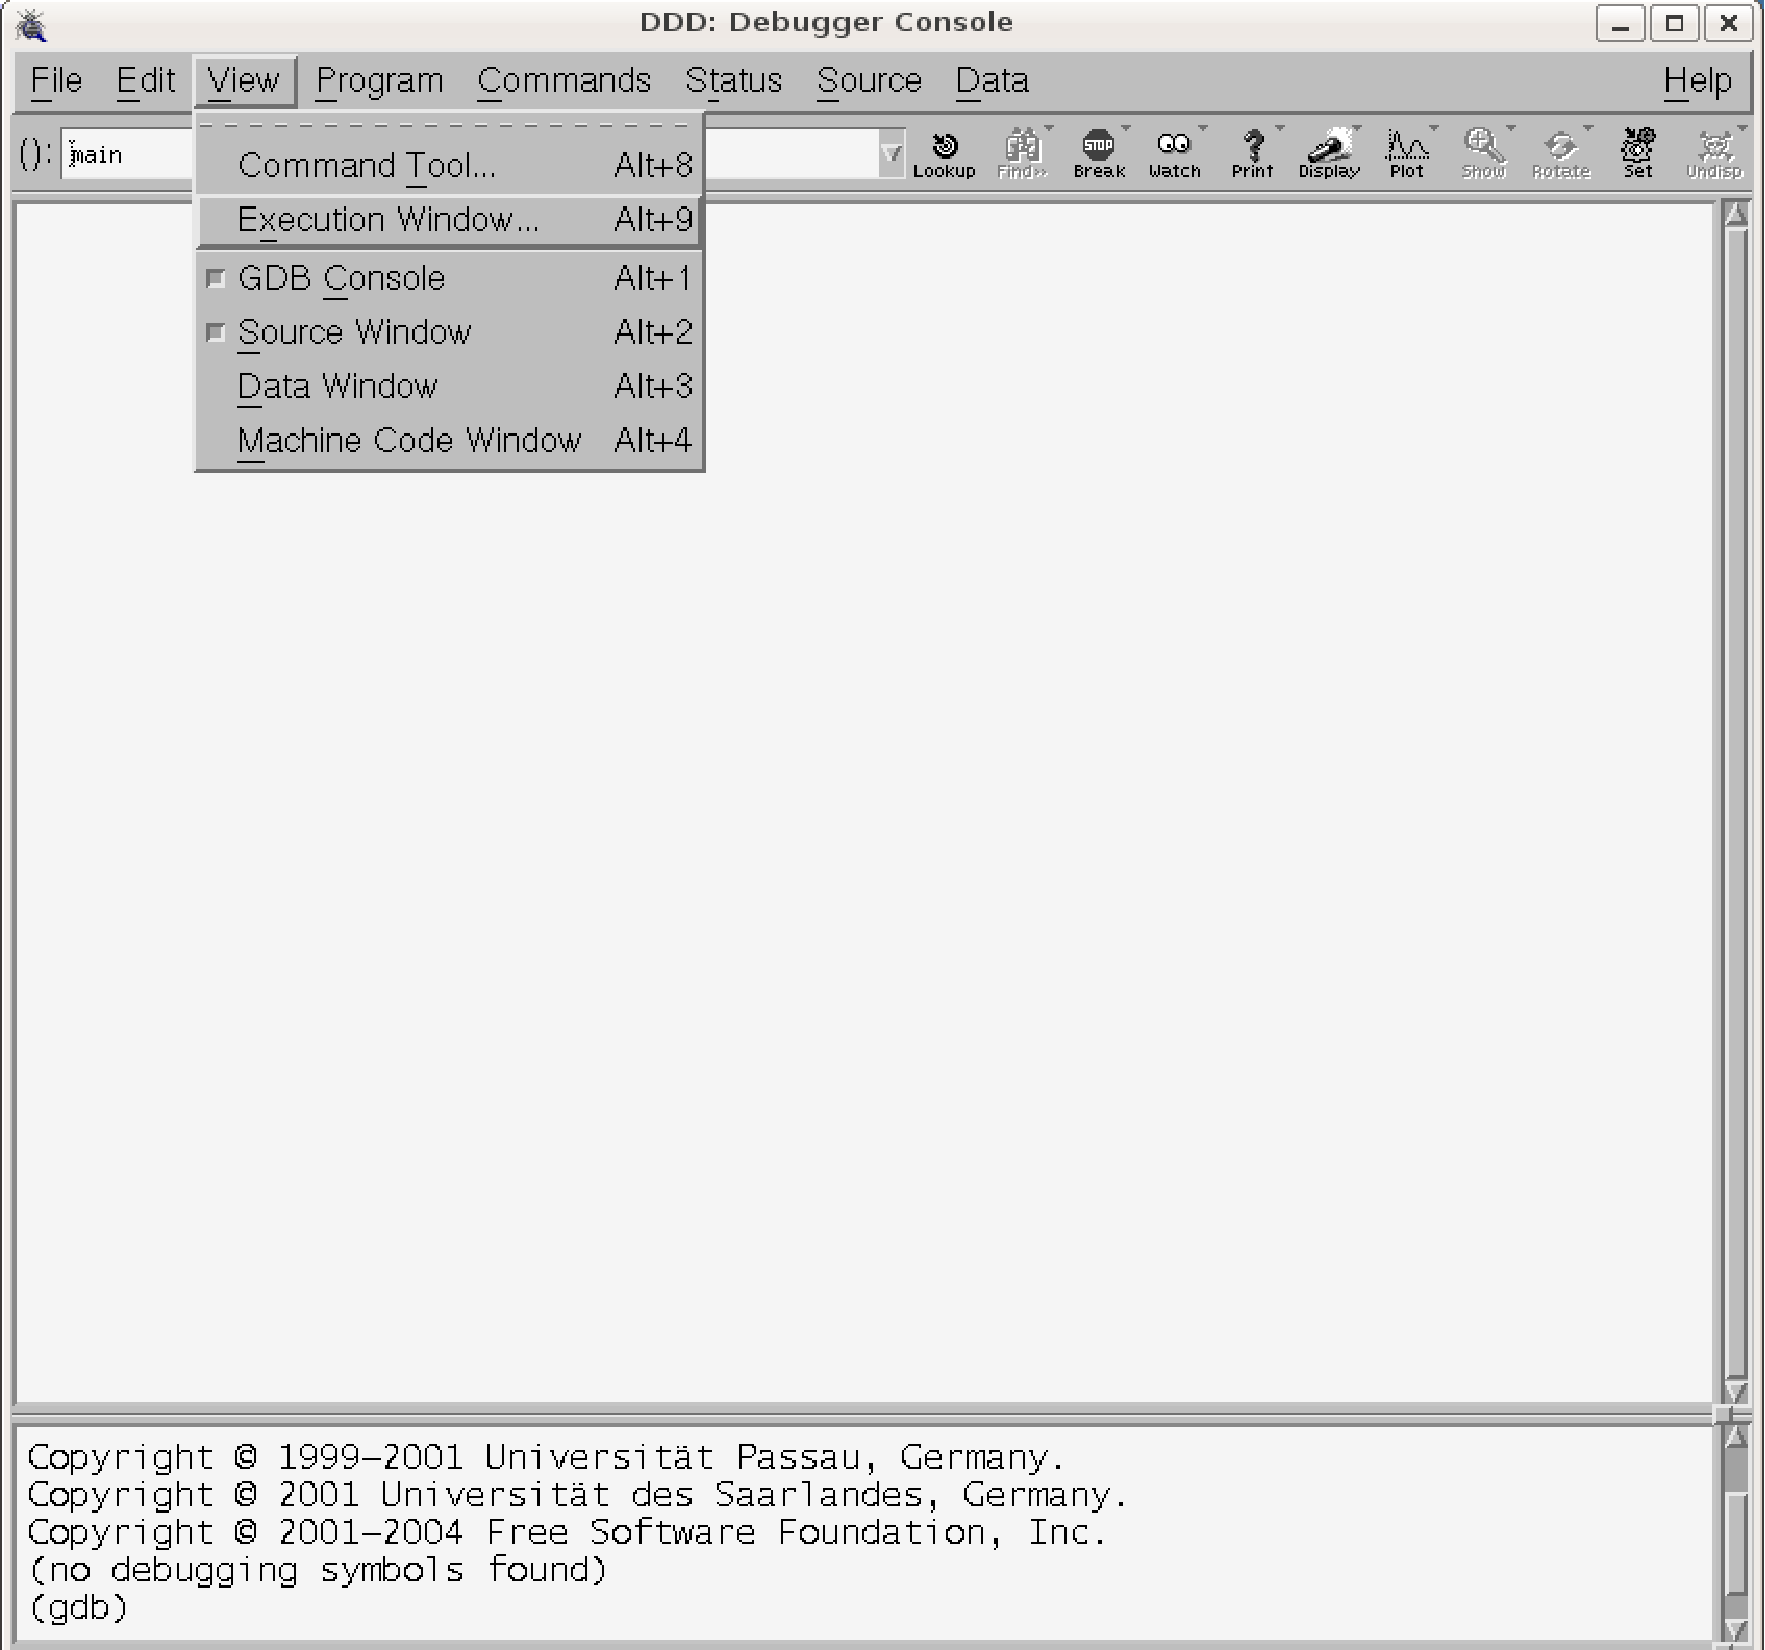
\includegraphics[width=8cm]{chapters/mardal-2/pdf/fig1.pdf}} \\
  \subfloat{ 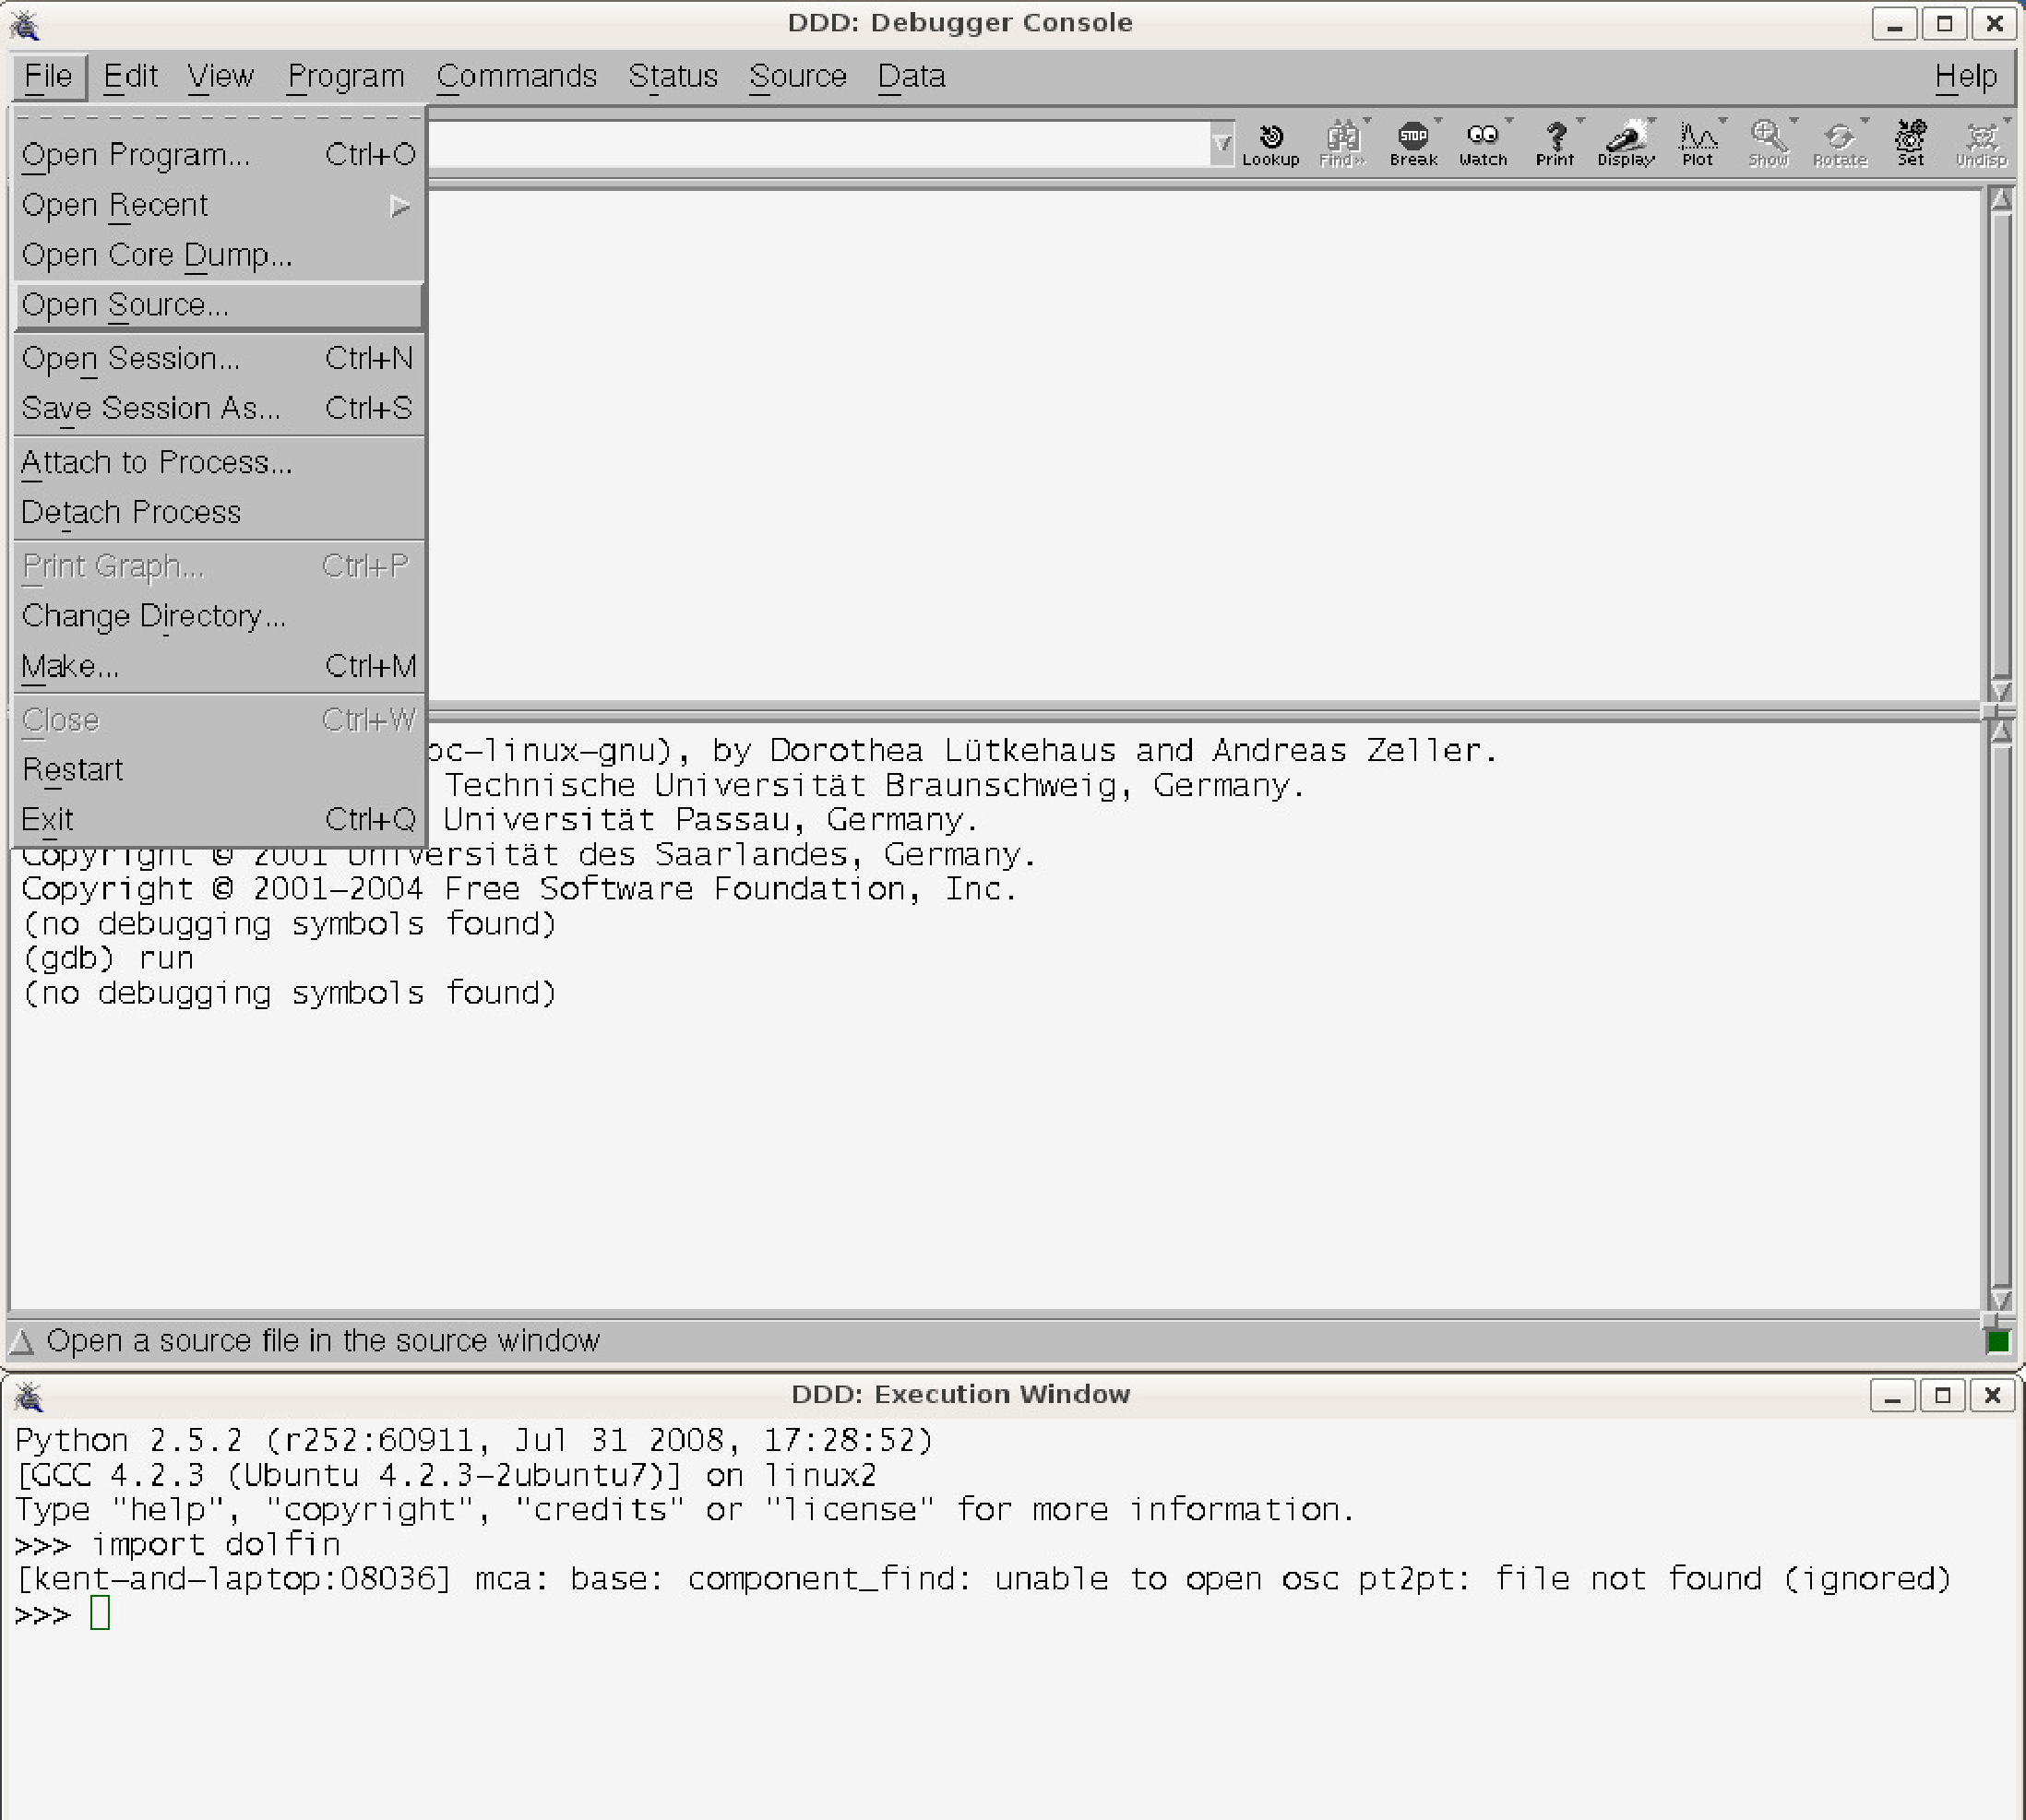
\includegraphics[width=8cm]{chapters/mardal-2/pdf/fig2.pdf}}
  \caption{Upper Picture: Starting a separate thread for the Python session in ddd.
           Lower Picture: Opening the source code after the \dolfin library has been loaded into Python.}
  \label{figure12}
\end{figure}
\begin{figure}
  \subfloat{ 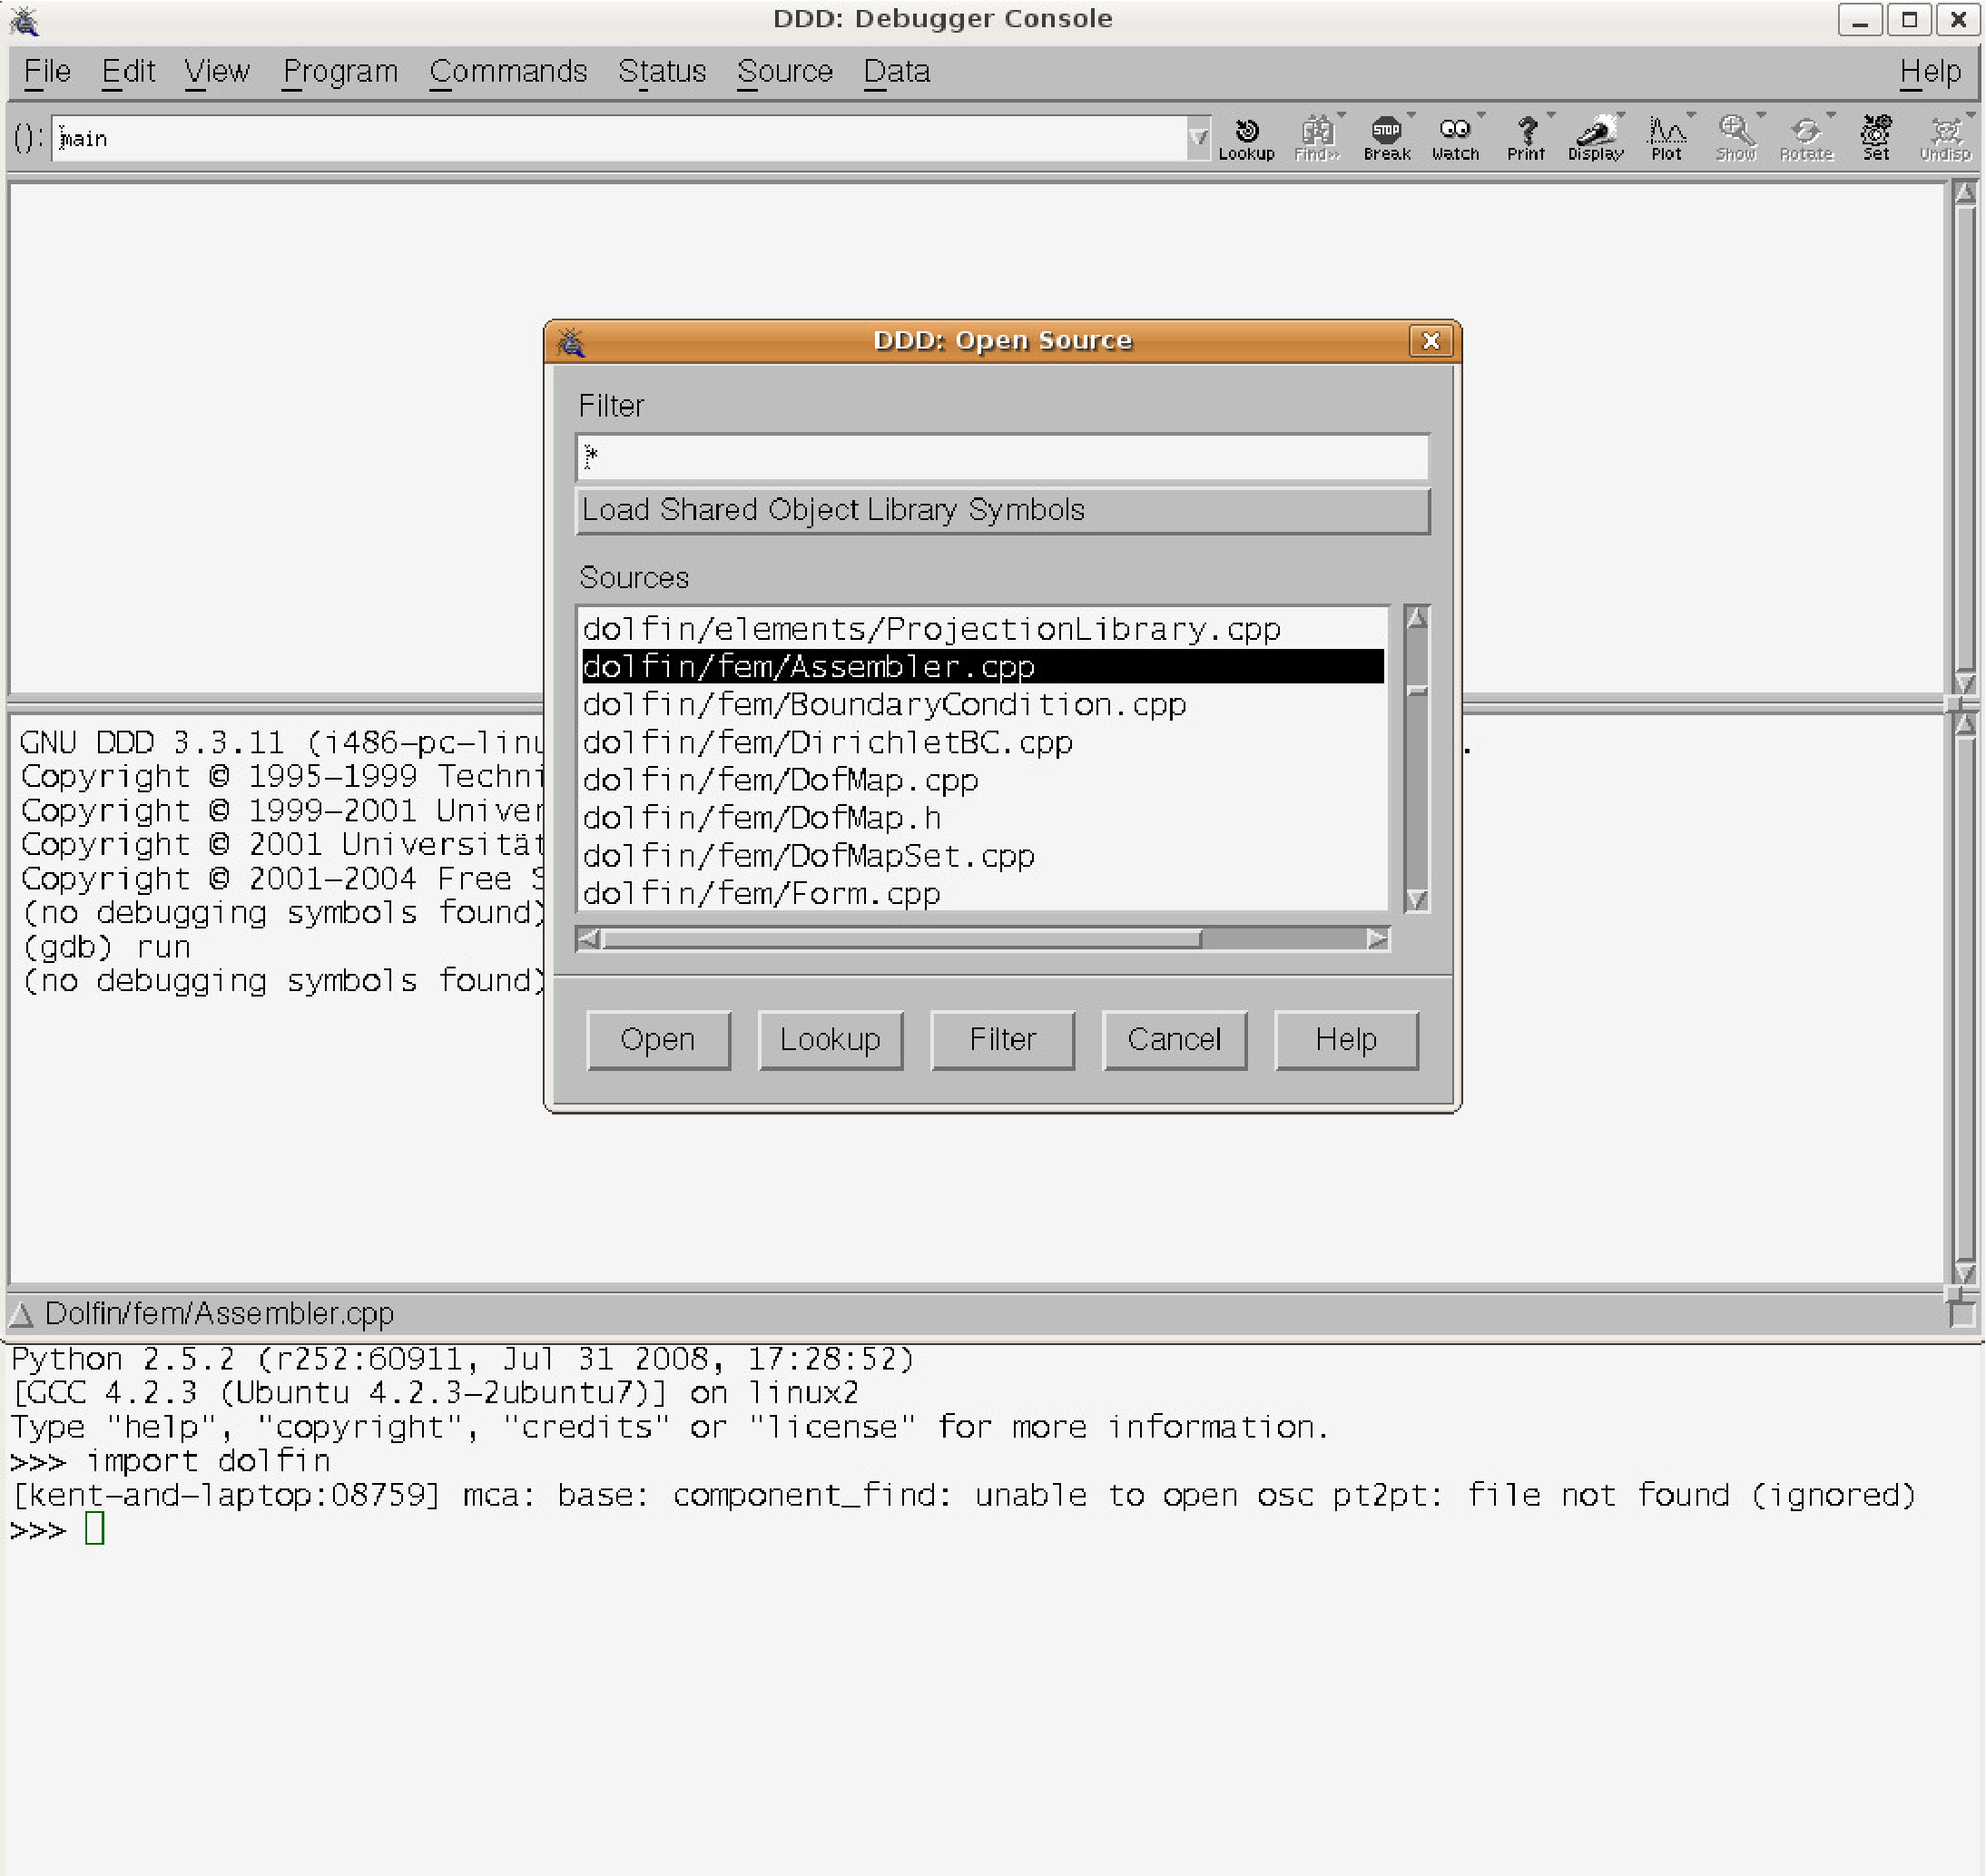
\includegraphics[width=8cm]{chapters/mardal-2/pdf/fig3.pdf}} \\
  \subfloat{ 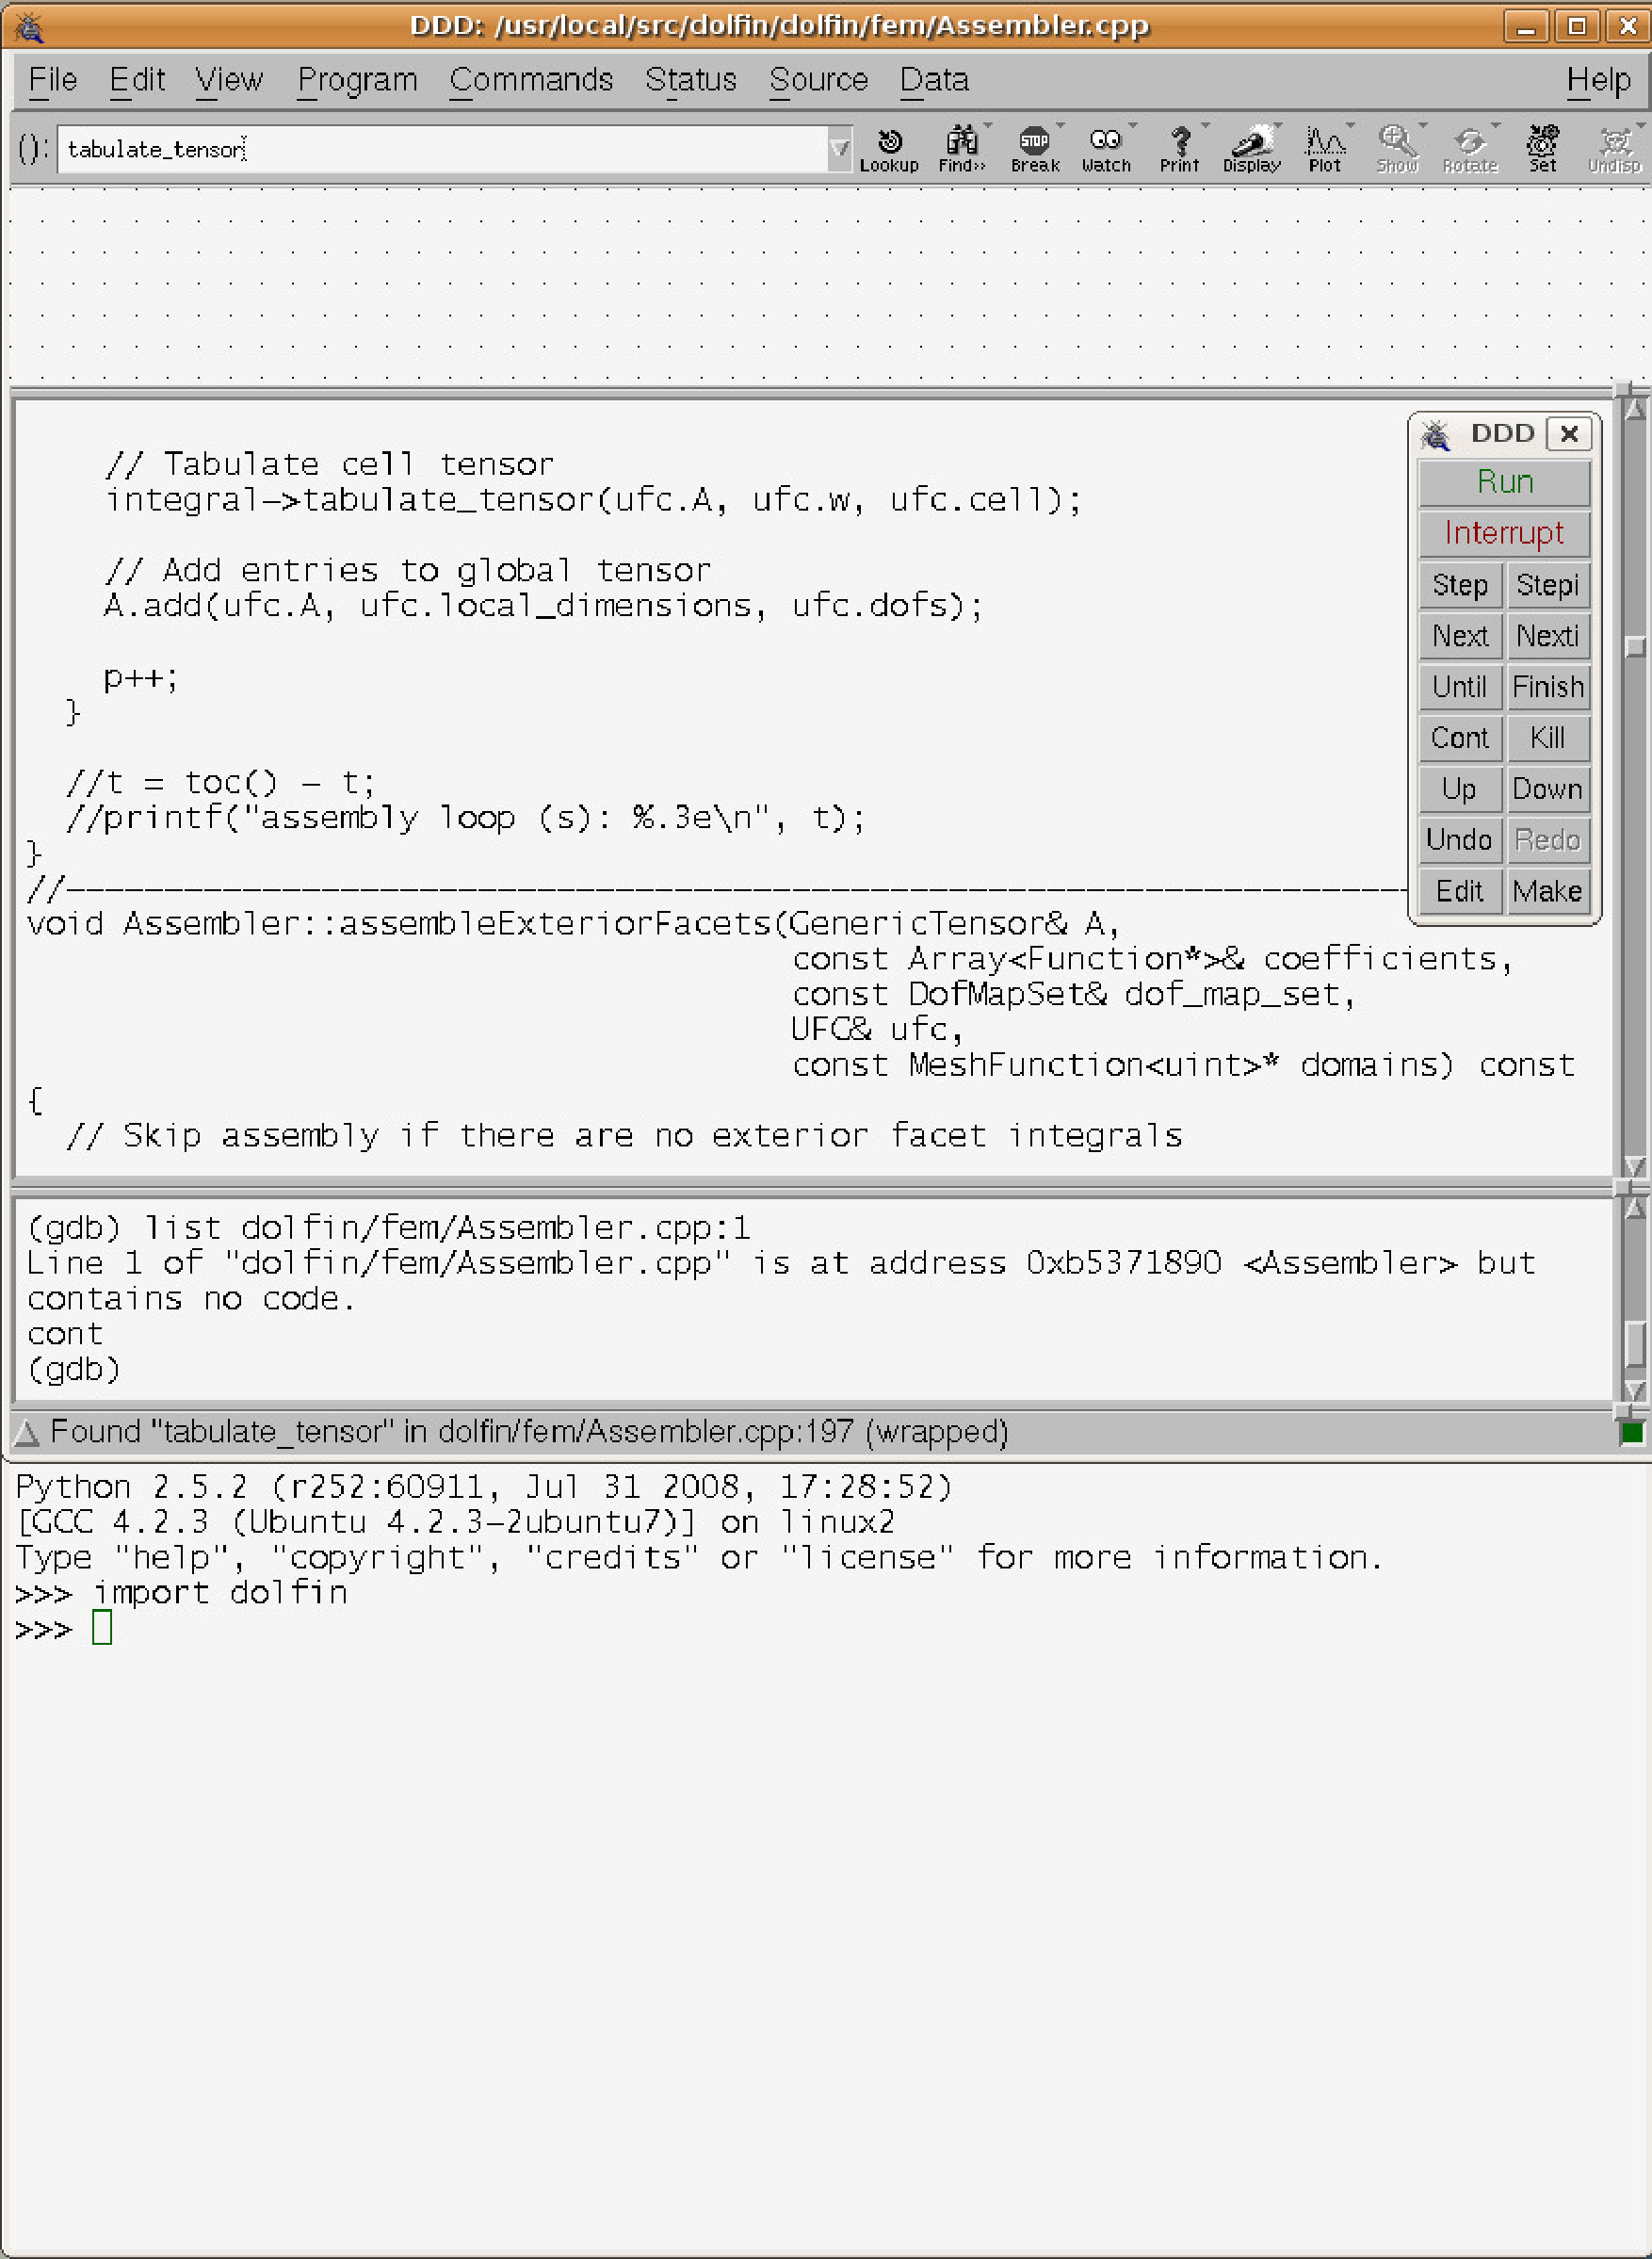
\includegraphics[width=8cm]{chapters/mardal-2/pdf/fig4.pdf}}
\caption{Upper Picture: Navigating through the source code for finding the assembly loop.
         Lower Picture: Searching for the function \emp{tabulate\_tensor.} }
\label{figure34}
\end{figure}

\begin{figure}
  \subfloat{ 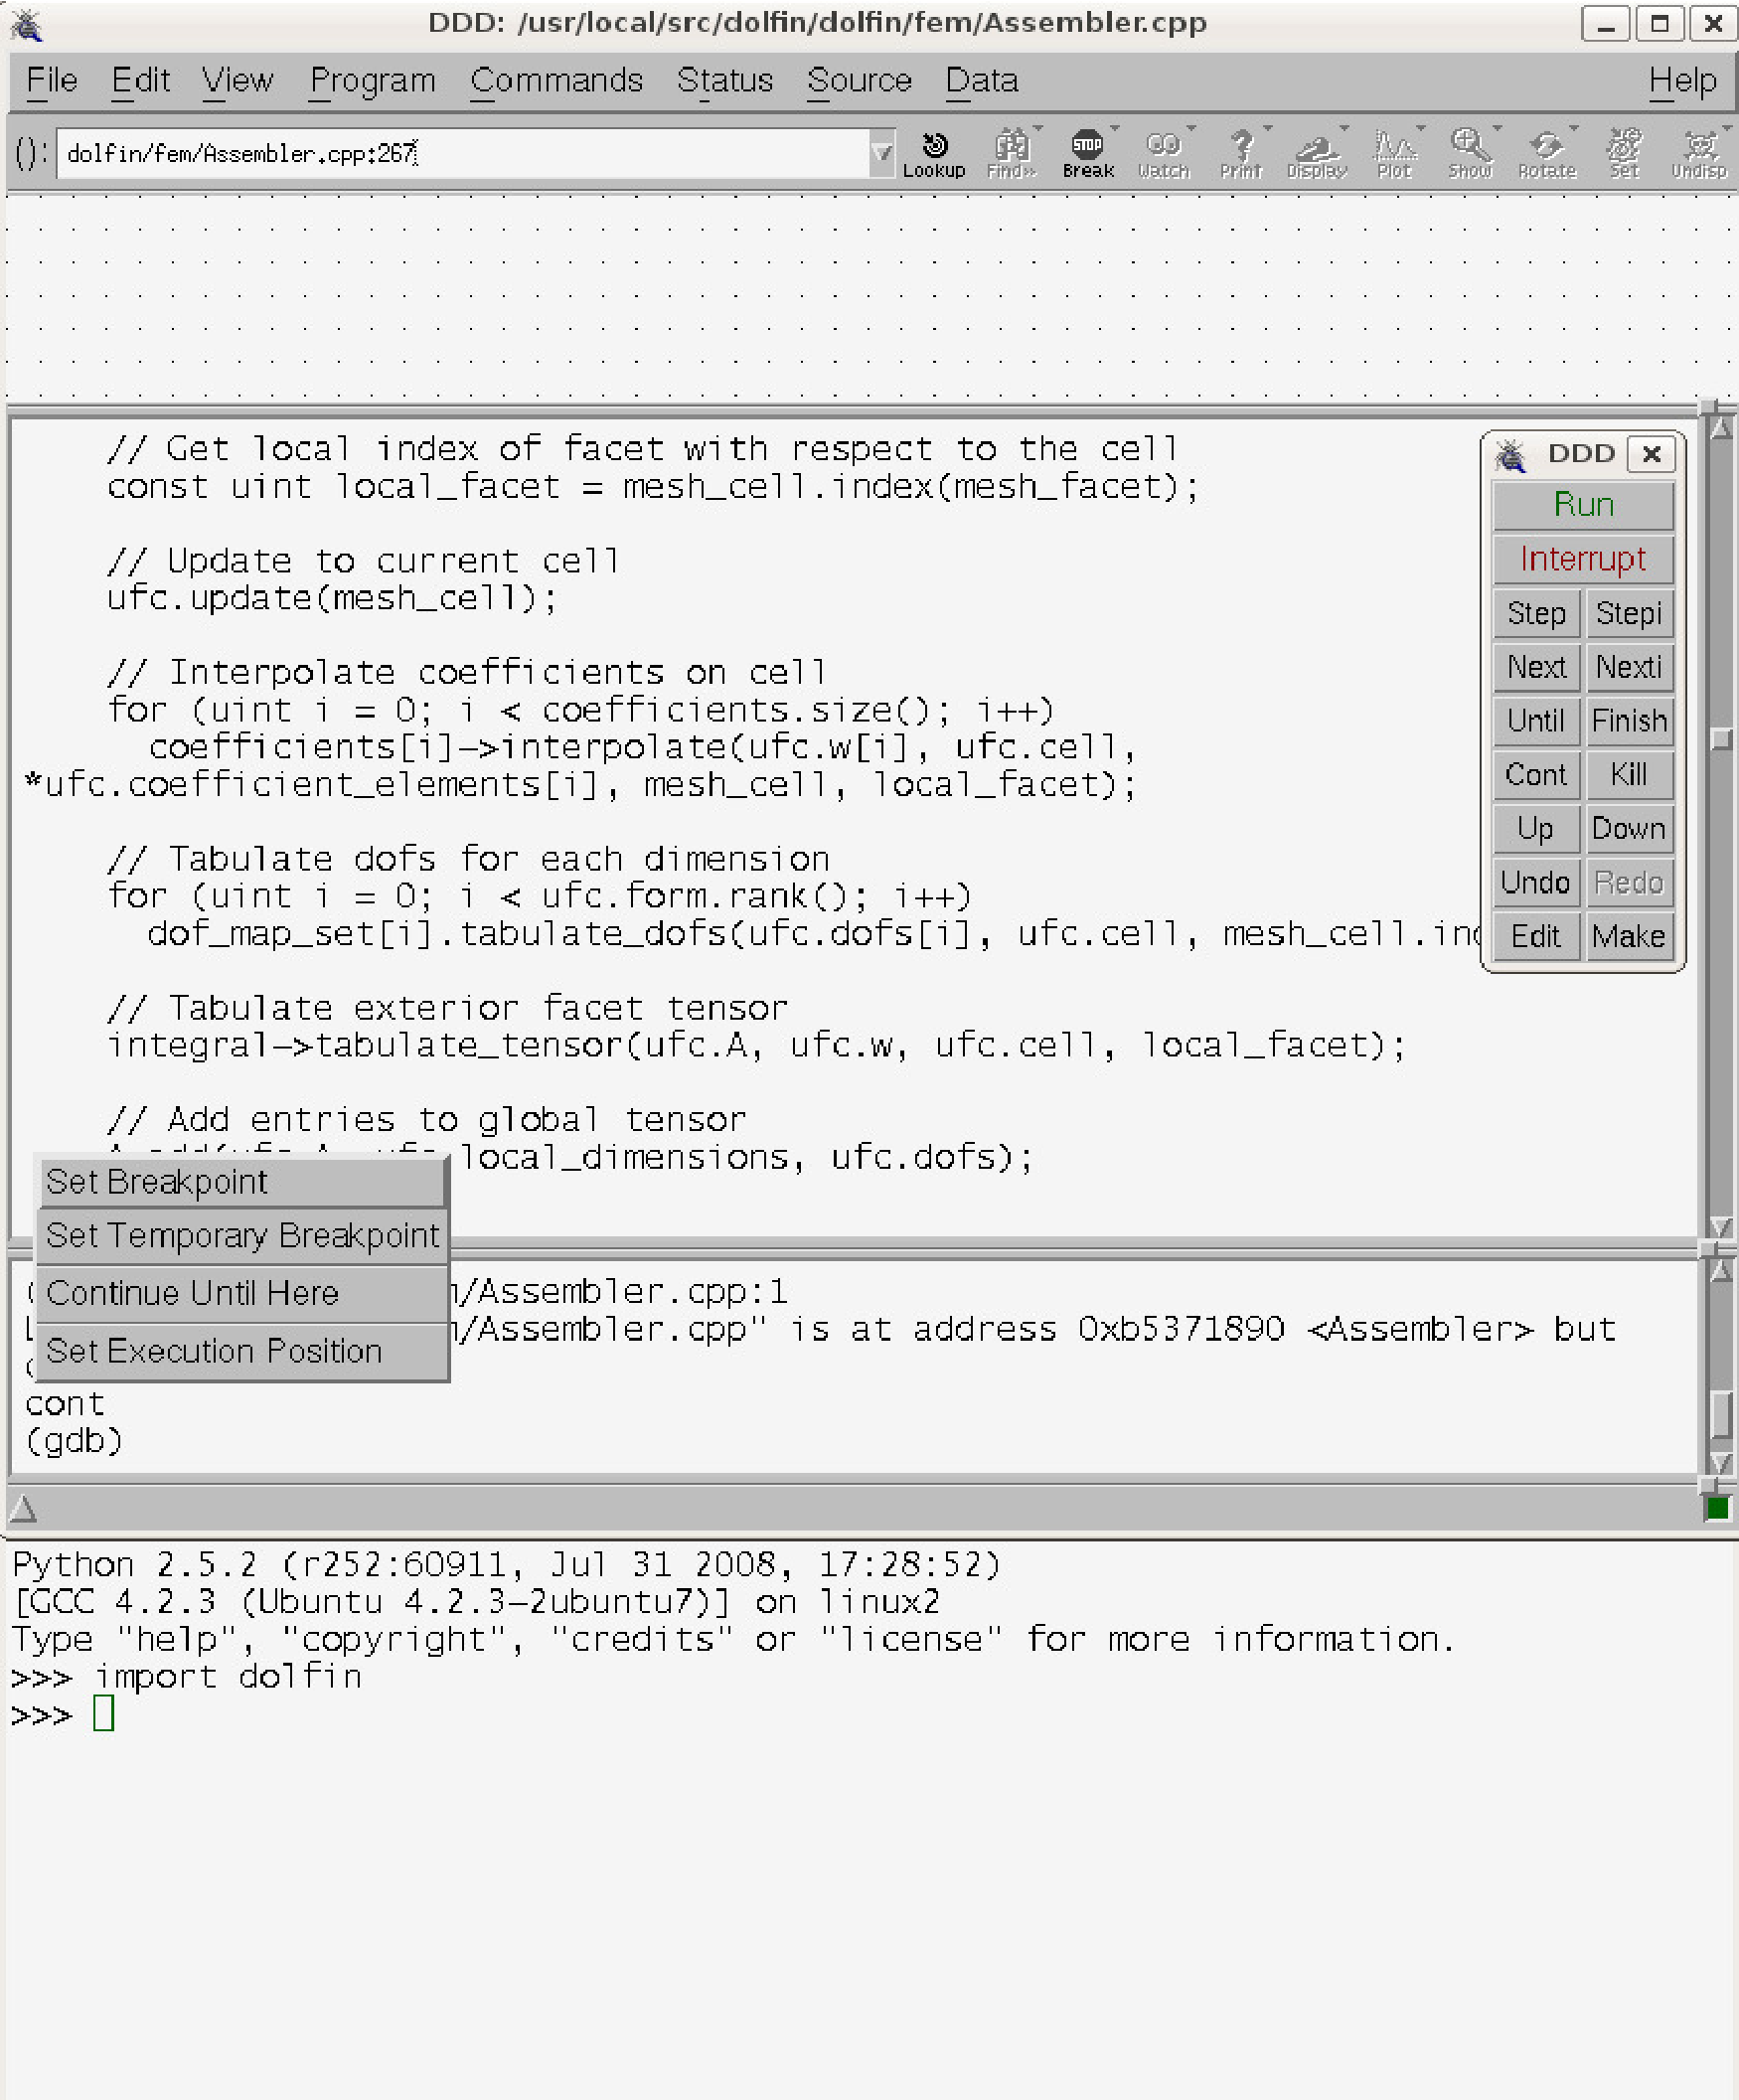
\includegraphics[width=8cm]{chapters/mardal-2/pdf/fig5.pdf}} \\
  \subfloat{ 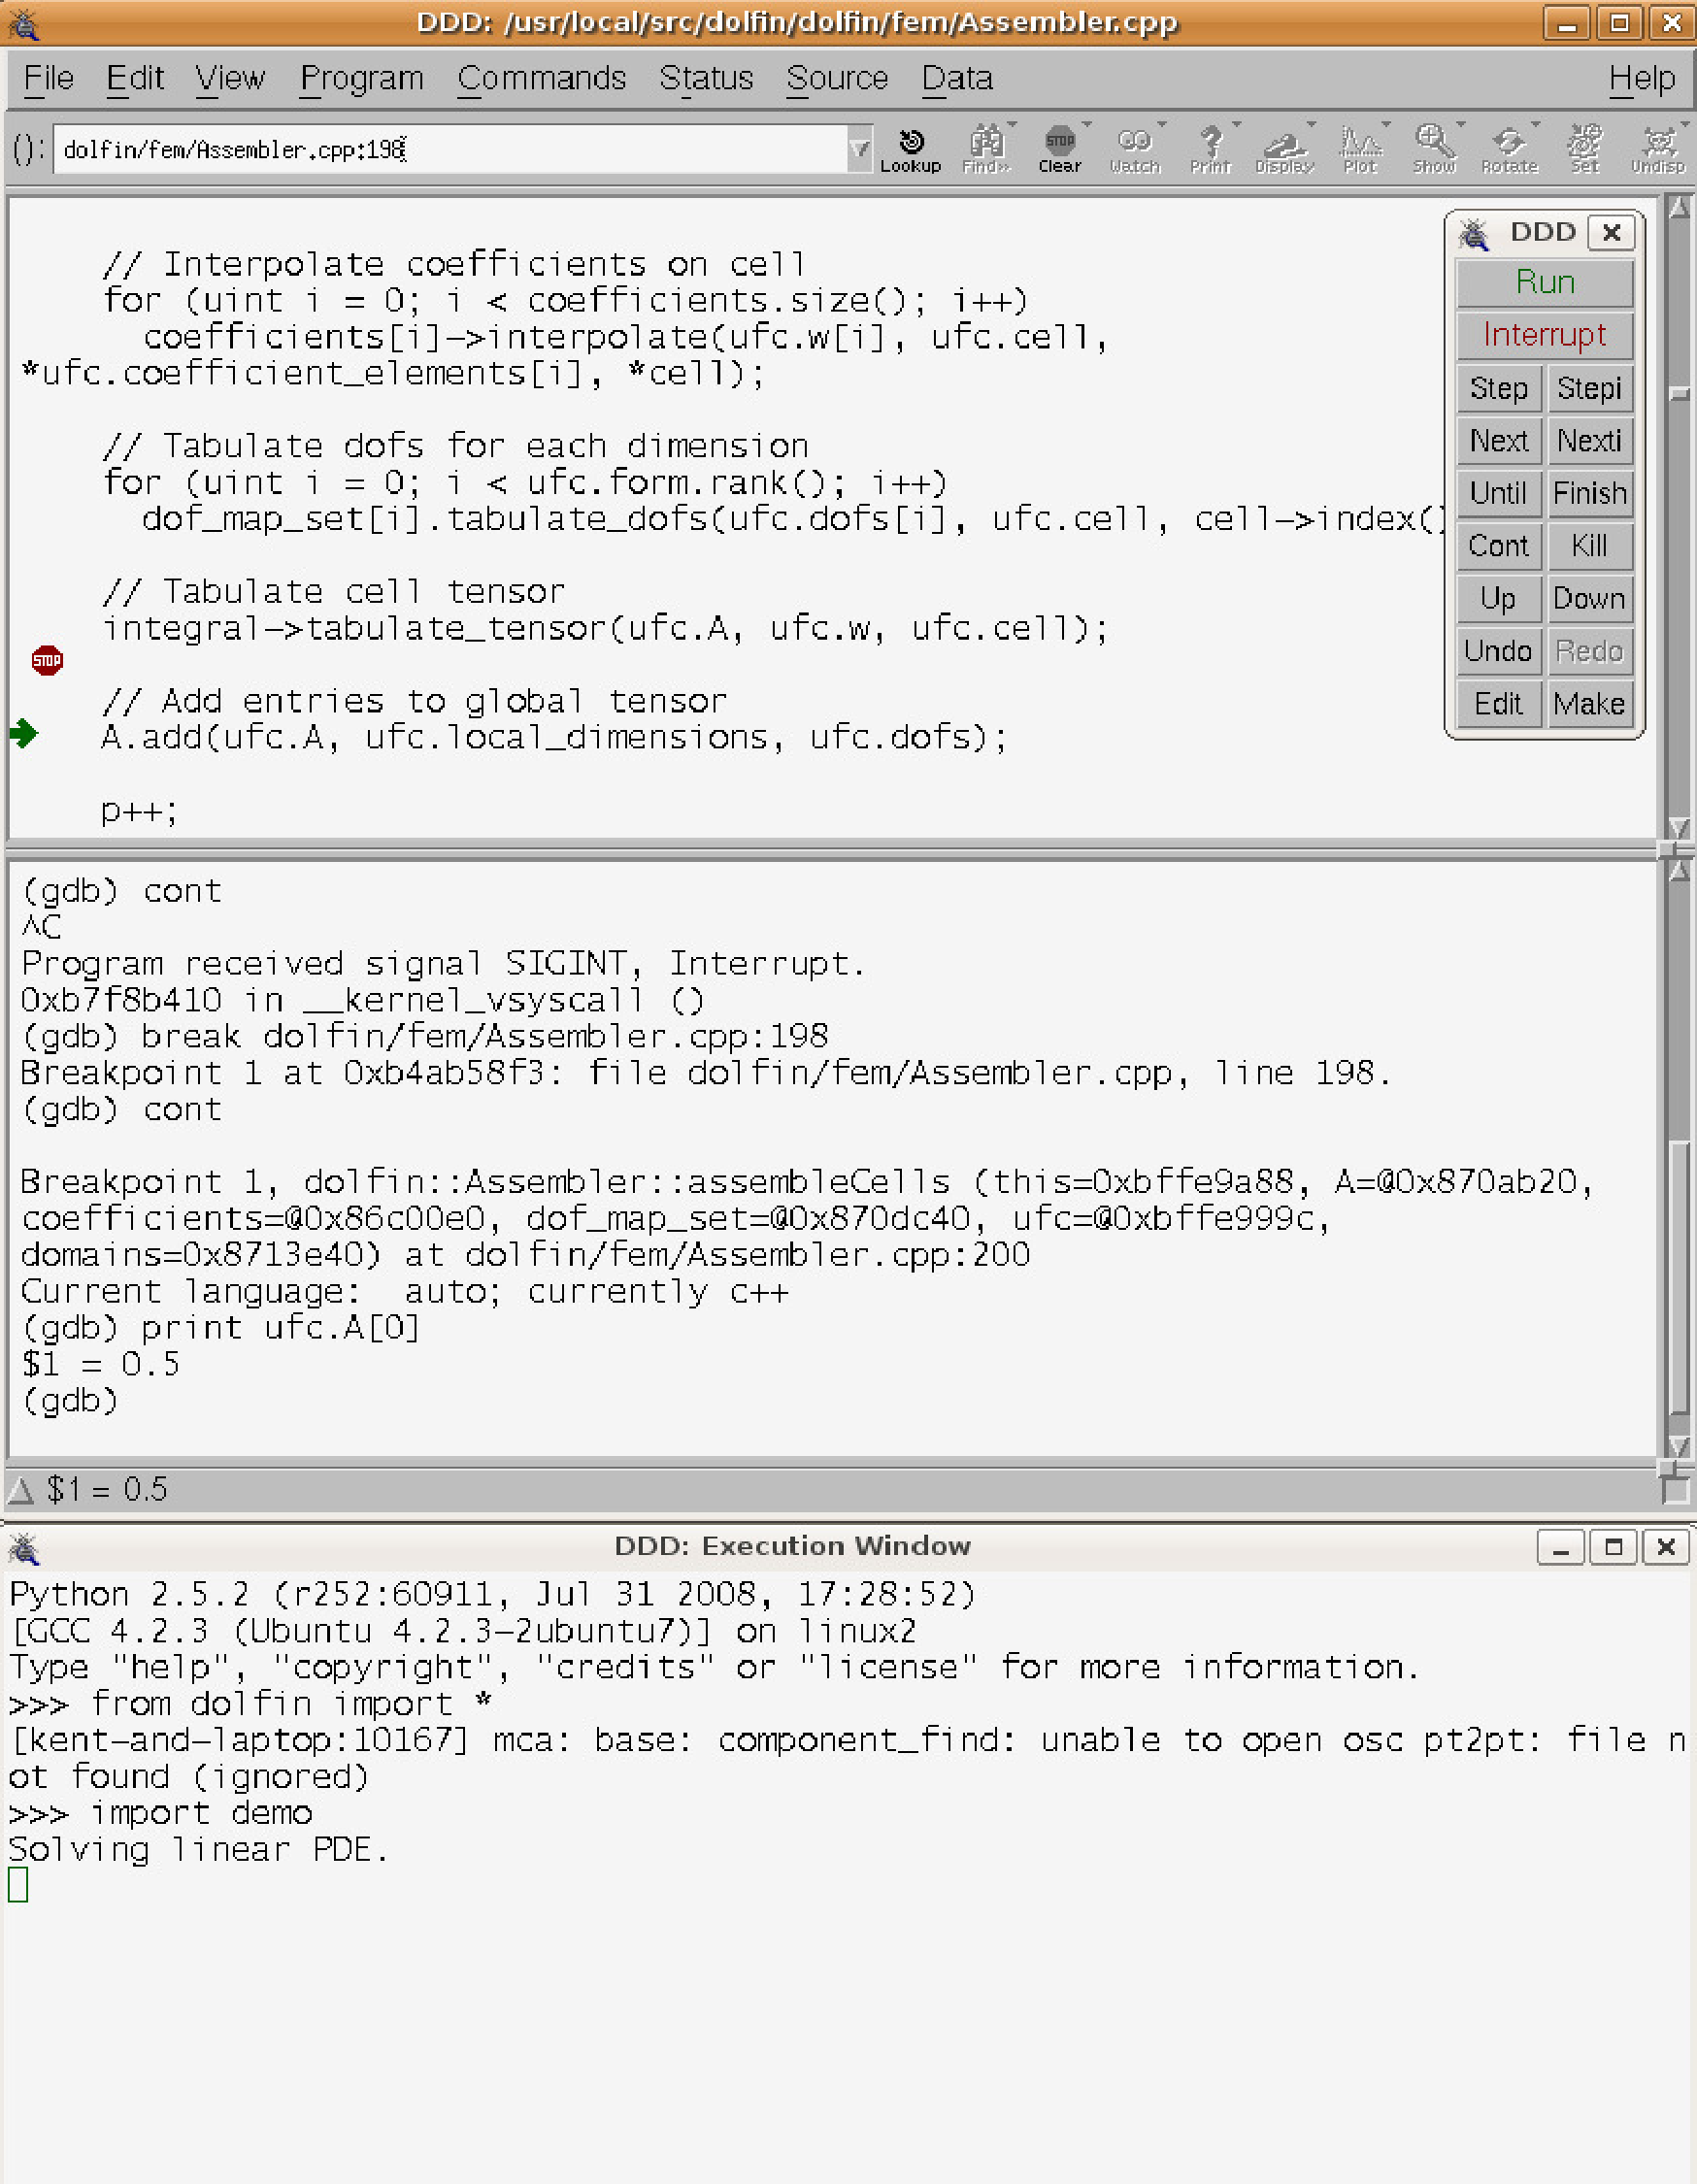
\includegraphics[width=8cm]{chapters/mardal-2/pdf/fig6.pdf}}
\caption{Setting a breakpoint after tabulate tensor and printing out the first element matrix entry.}
\label{fig5}
\end{figure}

\paragraph{Acknowledgments.}
The authors are very thankful to Johan Jansson who initiated the use of SWIG to wrap \dolfin to Python. We are also thankful to Ola Skavhaug who substantially extended the amount of \dolfin that got wrapped to Python and to Martin Alnaes who contributed to the JIT compilations of \emp{Expressions} and \emp{SubDomains}.

%%% Local Variables:
%%% mode: latex
%%% TeX-master: "../../book"
%%% End:
